%%%%%%%%%%%%%%%%%%%%%%%%%%%%%%%%%%%%%%%%%
% Short Sectioned Assignment LaTeX Template Version 1.0 (5/5/12)
% This template has been downloaded from: http://www.LaTeXTemplates.com
% Original author:  Frits Wenneker (http://www.howtotex.com)
% License: CC BY-NC-SA 3.0 (http://creativecommons.org/licenses/by-nc-sa/3.0/)
%%%%%%%%%%%%%%%%%%%%%%%%%%%%%%%%%%%%%%%%%

% \documentclass[paper=a4, fontsize=11pt]{scrartcl} % A4 paper and 11pt font size
\documentclass[11pt, a4paper]{book}
\usepackage[T1]{fontenc} % Use 8-bit encoding that has 256 glyphs
\usepackage[utf8]{inputenc}
\usepackage{fourier} % Use the Adobe Utopia font for the document - comment this line to return to the LaTeX default
\usepackage{listings} % para insertar código con formato similar al editor
\usepackage[spanish, es-tabla]{babel} % Selecciona el español para palabras introducidas automáticamente, p.ej. "septiembre" en la fecha y especifica que se use la palabra Tabla en vez de Cuadro
\usepackage{url} % ,href} %para incluir URLs e hipervínculos dentro del texto (aunque hay que instalar href)
\usepackage{graphics,graphicx, float} %para incluir imágenes y colocarlas
\usepackage[gen]{eurosym} %para incluir el símbolo del euro
\usepackage{cite} %para incluir citas del archivo <nombre>.bib
\usepackage{enumerate}
\usepackage{hyperref}
\usepackage{graphicx}
\usepackage{tabularx}
\usepackage{booktabs}
\usepackage[shortlabels]{enumitem} %enumerados personalizados
\usepackage{listings}
\usepackage[table,xcdraw]{xcolor} %para incluir colores en tablas
\usepackage[export]{adjustbox}  %para posicionar
\usepackage{svg} %para svg
\usepackage{textcomp}
\usepackage{subfiles} % Best loaded last in the preamble
\usepackage[bottom]{footmisc} % Lleva la nota a pie de página abajo el todo
\usepackage{appendix}
\usepackage{biblatex}
\addbibresource{bibliografia.bib}

\hypersetup{
	colorlinks=true,	% false: boxed links; true: colored links
	linkcolor=black,	% color of internal links
	urlcolor=cyan		% color of external links
}
\renewcommand{\familydefault}{\sfdefault}
\usepackage{fancyhdr} % Custom headers and footers
\pagestyle{fancyplain} % Makes all pages in the document conform to the custom headers and footers
\fancyhead[L]{} % Empty left header
\fancyhead[C]{} % Empty center header
\fancyhead[R]{Antonio Jiménez Rodríguez} % My name
\fancyfoot[L]{} % Empty left footer
\fancyfoot[C]{} % Empty center footer
\fancyfoot[R]{\thepage} % Page numbering for right footer
%\renewcommand{\headrulewidth}{0pt} % Remove header underlines
\renewcommand{\footrulewidth}{0pt} % Remove footer underlines
\setlength{\headheight}{13.6pt} % Customize the height of the header

\usepackage{titlesec, blindtext, color}
\definecolor{gray75}{gray}{0.75}
\newcommand{\hsp}{\hspace{20pt}}
\titleformat{\chapter}[hang]{\Huge\bfseries}{\thechapter\hsp\textcolor{gray75}{|}\hsp}{0pt}{\Huge\bfseries}
\setcounter{secnumdepth}{4}
\usepackage[Lenny]{fncychap}


\begin{document}

	% Plantilla portada UGR
	\begin{titlepage}
\newlength{\centeroffset}
\setlength{\centeroffset}{-0.5\oddsidemargin}
\addtolength{\centeroffset}{0.5\evensidemargin}
\thispagestyle{empty}

\noindent\hspace*{\centeroffset}\begin{minipage}{\textwidth}

\centering

\includegraphics[width=0.9\textwidth]{logos/logo_ugr.jpg}\\[1.4cm]

\textsc{ \Large TRABAJO FIN DE GRADO\\[0.2cm]}
\textsc{ GRADO EN INGENIERIA INFORMATICA}\\[1cm]

{\Huge\bfseries Título \\}
\noindent\rule[-1ex]{\textwidth}{3pt}\\[3.5ex]
{\large\bfseries Subtítulo }
\end{minipage}

\vspace{2.5cm}
\noindent\hspace*{\centeroffset}
\begin{minipage}{\textwidth}
\centering

\textbf{Autor}\\ {Estudiante}\\[2.5ex]
\textbf{Director}\\ {Tutor(a)(es)}\\[2cm]

\includegraphics[width=0.3\textwidth]{logos/etsiit_logo.png}\\[0.1cm]
\textsc{Escuela Técnica Superior de Ingenierías Informática y de Telecomunicación}\\
\textsc{---}\\
Granada, Junio de 201x
\end{minipage}
\end{titlepage}


	% Plantilla prefacio UGR
	\thispagestyle{empty}

\begin{center}
{\large\bfseries Título \\ Subtítulo }\\
\end{center}
\begin{center}
Nombre Del Estudiante\\
\end{center}

%\vspace{0.7cm}

\vspace{0.5cm}
\noindent{\textbf{Palabras clave}: \textit{software libre}
\vspace{0.7cm}

\noindent{\textbf{Resumen}\\
	

\cleardoublepage

\begin{center}
	{\large\bfseries Same, but in English}\\
\end{center}
\begin{center}
	Student's name\\
\end{center}
\vspace{0.5cm}
\noindent{\textbf{Keywords}: \textit{open source}, \textit{floss}
\vspace{0.7cm}

\noindent{\textbf{Abstract}\\


\cleardoublepage

\thispagestyle{empty}

\noindent\rule[-1ex]{\textwidth}{2pt}\\[4.5ex]

D. \textbf{Tutora/e(s)}, Profesor(a) del ...

\vspace{0.5cm}

\textbf{Informo:}

\vspace{0.5cm}

Que el presente trabajo, titulado \textit{\textbf{Chief}},
ha sido realizado bajo mi supervisión por \textbf{Estudiante}, y autorizo la defensa de dicho trabajo ante el tribunal
que corresponda.

\vspace{0.5cm}

Y para que conste, expiden y firman el presente informe en Granada a Junio de 2018.

\vspace{1cm}

\textbf{El/la director(a)/es: }

\vspace{5cm}

\noindent \textbf{(nombre completo tutor/a/es)}

\chapter*{Agradecimientos}






	% Índice de contenidos
	\newpage
	\tableofcontents

	% Índice de imágenes y tablas
	\newpage
	\listoffigures

	% Si hay suficientes se incluirá dicho índice
	\listoftables 
	\newpage

	% Introducción 
	\chapter{Introducción}

Este proyecto es software libre, y está liberado con la licencia \cite{gplv3}.

Debido a la situación tan extraordinaria que hemos vivido en estos últimos años con la Covid-19
muchas de nuestra actividades y negocios han sufrido cambios bastante notables.
Por ejemplo el tele-trabajo en las empresas privadas, aparentemente ha llegado para
quedarse y dar así al trabajador una mayor libertad de movimiento con el objetivo de
aumentar su comodidad y productividad.

Otros de los sectores afectados han sido los negocios de citas. Estos se vieron obligados
a trabajar únicamente con cita previa debido a la prohibición de poder haber varias personas
esperando en una sala de espera o en la propia sala del negocio.

Ante este problema surge la necesidad de crear un aplicativo que gestione de una manera
sencilla todo lo relacionado con la reserva de citas y que ayude a los usuarios de estos negocios en el proceso.

	% Descripción del problema y hasta donde se llega
	\chapter{Descripción del problema}

Dado un caso real, en donde a una barbería normalmente acudía la gente sin previo aviso para esperar a
poder ser atendida, tuvo que adaptarse a las nuevas normativas y habilitar un teléfono para la reserva de citas.

Se plantea a partir de esta situación, la creación de una aplicación web/móvil que permita la gestión de las citas
automáticamente, sin necesidad de que el trabajador se distraiga de su labor. Facilitando también a los usuarios la
consulta de horarios y disponibilidad del mismo, permitiendo elegir la fecha deseada con unas simples acciones,
además de tener un registro de las diferentes reservas.

	% Estado del arte
	% 	1. Crítica al estado del arte
	% 	2. Propuesta
	\chapter{Análisis del Sistema}

Este sistema a implementar pretende resolver el posible problema de un negocio de cita previa a saltar al terreno online.

Se desarrollará un sistema donde un cliente del mismo solo tenga que completar la información requerida en la base de datos del aplicativo. Mediante un despliegue de un nuevo entorno, que será realizado por los programadores, se obtendrá una nueva página web totalmente funcional en la que dicho negocio podrá tener a sus clientes identificados y ofrecerles la posibilidad de la reserva de citas o de compra de producto de una manera más cómoda desde casa.

\section{Casuísticas}

Al ser un sistema que intenta abarcar varios frentes bastantes amplios existen muchas casuísticas que se podrían dar en el aplicativo.

\subsection{Acceso al público}

Está claro que el objetivo principal es llegar a una mayor cantidad de personas y dar el negocio a conocer por la red. Sin embargo, no se puede proporcionar una web en la que todos los sitios sean accesibles por cualquier persona. Para esto se va a implementar un sistema de usuarios por negocio. Un usuario sin identificarse tendrá acceso a la página de presentación del negocio y a la página de productos de la tienda. Por el contrario, sin autenticación no se le dará acceso a la reserva de citas ni a la realización de pedidos online. Con esto también conseguimos quitar una carga al servidor de Back-End, ya que por ejemplo, para un usuario nuevo que aún no se ha registrado en el negocio no se harán peticiones desde las webs al servidor para la obtención de todos estos datos.

\subsubsection{Ataques al sistema}

Debido al acceso público se pueden dar casos de ataques al sistema. En internet se realizan miles y miles de ataques cibernéticos al segundo y nuestro sistema no tiene por qué ser una excepción. Para ello se tendrá especial atención en el trato de datos de inserción en el sistema y se validarán los usuarios registrados con el fin de intentar filtrar lo máximo posible a los usuarios reales de los que no lo son.

\subsection{Reserva de citas}

Otro de los bloques principales es la reserva de cita previa. Aquí se debe conseguir no romper la organización del propio negocio, no dándole la posibilidad a un cliente que reserve a una hora y minuto exacto a la que él desee ser atendido, sino que los clientes deberán seleccionar las horas que vienen definidas por el propio negocio. Parece obvio, pero una mala gestión de esta parte podría causar un caos en el sistema y en el propio negocio a la hora de atender a estos clientes.

Para ello se realizarán todas las comprobaciones y validaciones necesarias antes (al mostrar las citas disponibles a los clientes) y después (una vez el cliente haya enviado su reserva) para no cometer ningún error ni colapso.

\subsubsection{Cancelación de citas}

Este frente puede ser problema para el negocio, ya que cualquiera podría registrarse con sus datos, realizar una reserva de una cita online y cancelarla cinco minutos antes de tener que ser atendido. Para evitar esto se deberá implementar funcionalidades para que un usuario pueda cancelar una cita dentro de un límite establecido. Si aun así el cliente no asiste a la cita por un motivo no justificado esta deberá poder ser marcada para una posible penalización.

\subsection{Compra de productos}

El último gran bloque de este sistema es la compra de productos online ofertados por cada negocio. Desde el sistema y las diferentes webs se podrá acceder a un catálogo de productos gestionado por cada negocio en la que los usuarios podrán crear un carrito de la compra y procesar su pedido. Además tendrá acceso al estado y seguimiento de este. Los pagos deberán gestionarse por alguna herramienta externa que de soporte para ello y se adaptará la información almacenada en base de datos para los datos proporcionados por la herramienta elegida.

\section{Tipos de usuarios}

Para este sistema se definirán tres tipos de usuarios los cuales podrán interactuar con él de diferente forma debido a los permisos de accesibilidad.

\subsubsection{Superadministrador}

Este usuario será el que controle todo el aplicativo completo teniendo acceso al total de los datos almacenados en la base de datos. Podrá ver, modificar o eliminar datos si así lo ve oportuno, ya sea por errores producidos o por peticiones de los jefes de los negocios. Además será el encargado de revisar las notificaciones de errores que se registren y deberá mantener el orden en el funcionamiento de cada negocio.

\subsubsection{Trabajadores}

Ellos tendrán acceso completo a los datos almacenados a nivel de negocio. Podrán consultar las citas o pedidos realizados por los siguientes usuarios y notificar a un superadministrador en caso de que se haya encontrado alguna anomalía. Podrán reservar citas para clientes ya registrados o en su defecto reservar citas con el número del cliente que lo desee. Si por ejemplo, una persona mayor que no se maneje bien con el mundo de internet desea una cita en el negocio, el trabajador podría reservar una cita con el número de teléfono del cliente sin necesidad de que este esté previamente registrado.

\subsubsection{Clientes}

El cliente es el usuario encargado de que el sistema tenga vida. Estos podrán registrarse en los distintos negocios (serán distintas cuentas por negocio), reservar citas previas y realizar pedidos de productos. Debido a que los clientes serán los encargados de alimentar la base de datos deberemos tener gran cuidado a la hora de tratar la información proporcionada para así evitar posibles ataques o errores humanos. Esto lo podemos conseguir sanitizando la información y validando los datos en tiempo real mostrándole al usuario los posibles errores cometidos.



	
	\chapter{Planificación}

\section{Metodología utilizada}

Para el desarrollo de este proyecto se ha elegido como metodología el \textbf{Desarrollo Ágil}.
En mi opinión, ete tipo de enfoque se acerca más al que desarrollan las empresas en la actualidad, donde se
definen sprints en los que los requisitos y soluciones van evolucionando según la necesidad del proyecto.
No obstante cada iteración deberá tener su planificación, análisis de requisitos, diseño, tests, etc.

\section{Temporización}

La temporización general de este proyecto va a estar dividida en dos: construcción del Web Service para la
gestión de los datos del aplicativo y la creación de un entorno Front-End para los usuarios. A su vez estos dos
objetivos principales estarán divididos en diferentes hitos para realizar un desarrollo progresivo.

\vspace{0.5em}
\begin{itemize}
    \item \textbf{Web Service}:
        \begin{itemize}
            \item \textbf{Gestión de citas previas}: En este primer hito se completará toda la funcionalidad referente
            a la gestión de cita previa. Contendrá todo lo necesario para que desde la aplicación Webs se puedan
            realizar operaciones como reserva de citas por parte de usuarios; obtención de histórico de citas ya
            sea del negocio, usuarios o trabajadores; cancelación de citas; así como todas las comprobaciones y
            controles para la gestión de estas citas. De la mano de este hito se completará también la gestión
            de inicio de sesión de usuario y la encriptación de datos privados en la base de datos del aplicativo.

            \item \textbf{Dockerización e Integración Continua}: Este hito no hace aportación de nueva funcionalidad
            para el Web Service en construcción pero si es una parte esencial del proyecto. El objetivo de desplegar un
            contenedor docker de \textbf{tests} es poder tener una batería de test para la aplicación y mediante
            Github Actions, que será el Sistema de Integración Continua elegido, lanzar estos tests en los commits
            que se vayan realizando en el desarrollo del proyecto. Así nos aseguraremos que en toda nueva funcionalidad
            creada o mejoras de código se realizan las acciones deseadas.

            \item \textbf{Gestión de venta de productos online}: Una vez finalizadas las dos etapas anteriores
            pasaremos a desarrollar otro de los puntos principales del problema, la gestión de venta online de
            productos. En este hito se deberá implementar la gestión de los pedidos que lleguen desde la aplicación
            Front-End de los usuarios de las Webs.

            \item \textbf{Administración Back-End}: Por último se va a añadir para el Back-End desarrollado una vista
            de administración para poder acceder a todos los datos registrados por cada negocio. Además se podrán
            añadir funcionalidades para los trabajadores o un panel de estadísticas donde ver información relevante.
        \end{itemize}
    \item \textbf{Aplicación Web/Móvil}:
    \begin{itemize}
                \item \textbf{Esqueleto y Home}:

                \item \textbf{Interfaz para la reserva de citas}:

                \item \textbf{Interfaz para las compras online de productos}:

                \item \textbf{Interfaz para perfil de usuario}:
            \end{itemize}
\end{itemize}
\section{Seguimiento del desarrollo}


	% Análisis del problema
	% 1. Análisis de requisitos
	% 2. Análisis de las soluciones
	% 3. Solucion propuesta
	% 4. Análisis de seguridad
	\chapter{Análisis del problema}

\section{Implicados}

En esta sección vamos a centrarnos en los implicados del problema a resolver ya que estos serán los usuarios finales de
la aplicación. Definiremos a continuación los distintos tipos de usuario.

\subsection{Tipos de usuario}

Los usuarios potenciales de la aplicación son:

\begin{itemize}
    \item Super-Administrador. Su función es gestionar la totalidad del aplicativo, teniendo acceso total a los datos
    almacenados por cada uno de los negocios. Podrá monitorizar el correcto funcionamiento de la aplicación y realizar
    correcciones o registrar incidencias si es necesario.

    \item Trabajador. Su función es gestionar los datos de un negocio. En este caso el trabajador 
    tendrá acceso a los datos del mismo. Si detecta posibles errores también podrá registrar incidencias.

    \item Usuarios. Podrán consultar y reservar citas, así realizar pedidos en la tienda online.
    Además tendrán acceso a todos su datos como histórico de citas o histórico de pedidos.
\end{itemize}

\subsection{Resumen de implicados}

\begin{table}[H]
\begin{tabular}{|c|l|c|l|}
\hline
\textbf{Nombre} & \multicolumn{1}{c|}{\textbf{Descripción}} & \textbf{Tipo} & \multicolumn{1}{c|}{\textbf{Responsabilidad}} \\ \hline
Super-Administrador & \begin{tabular}[c]{@{}l@{}}Administrador \\ del sistema\end{tabular} & \begin{tabular}[c]{@{}c@{}}Usuario\\ producto\end{tabular} & \begin{tabular}[c]{@{}l@{}}Gestionar el sistema, moniro- \\ rizar sistema, gestionar inci- \\ dencias.\end{tabular} \\ \hline
Trabajador & \begin{tabular}[c]{@{}l@{}}Trabajador \\ del negocio\end{tabular} & \begin{tabular}[c]{@{}c@{}}Usuario\\ producto\end{tabular} & \begin{tabular}[c]{@{}l@{}}Gestionar el negocio, modificar \\ datos del negocio (citas, \\ productos,...), registrar \\ incidencias.\end{tabular} \\ \hline
Usuario & \begin{tabular}[c]{@{}l@{}}Cliente que \\ usa el sistema \\ de manera \\ convencional.\end{tabular} & \begin{tabular}[c]{@{}c@{}}Usuario\\ producto\end{tabular} & \begin{tabular}[c]{@{}l@{}}Reservar/modificar/cancelar \\ citas, realizar pedidos, \\ gestionar perfil de usuario.\end{tabular} \\ \hline
\end{tabular}
\caption{Resumen de implicados}
\end{table}

\subsection{Perfiles de los implicados}

\textbf{Administrador}

\begin{table}[H]
\begin{tabular}{|l|l|}
\hline
\textbf{Representante} & Nombre Apellidos \\ \hline
\textbf{Descripción} & Super-Administrador \\ \hline
\textbf{Tipo} & \begin{tabular}[c]{@{}l@{}}
Encargado del sistema completo, con responsabilidades\\ de gestión sobre el mismo.
\end{tabular} \\ \hline
\textbf{Responsabilidades} & \begin{tabular}[c]{@{}l@{}}
Gestionar el sistema correctamente: supervisar\\ los errores que puedan surgir en el aplicativo y controlar\\
el funcionamiento.
\end{tabular} \\ \hline
\textbf{Criterios de éxito} & \begin{tabular}[c]{@{}l@{}}
Que el sistema funcione adecuadamente con los pará-\\ metros óptimos y no exista información incorrecta.
\end{tabular} \\ \hline
\textbf{Implicación} &
Total, pues es el encargado principal del sistema. \\ \hline
\end{tabular}
\caption{Perfil de implicado: Super-Administrador}
\end{table}

\textbf{Trabajador}

\begin{table}[H]
\begin{tabular}{|l|l|}
\hline
\textbf{Representante} & Nombre Apellidos \\ \hline
\textbf{Descripción} & Administrador de negocio \\ \hline
\textbf{Tipo} & \begin{tabular}[c]{@{}l@{}}
Encargado del negocio al que pertenece, \\
con responsabilidades de gestión sobre el mismo.
\end{tabular} \\ \hline
\textbf{Responsabilidades} & \begin{tabular}[c]{@{}l@{}}
Gestionar su negocio: supervisar\\ y controlar los datos referentes a su negocio\\ para que no aparezcan incongruencias.
\end{tabular} \\ \hline
\textbf{Criterios de éxito} & \begin{tabular}[c]{@{}l@{}}
Que no se detecten errores en los datos almacenados.
\end{tabular} \\ \hline
\textbf{Implicación} &
Total a nivel de negocio. \\ \hline
\end{tabular}
\caption{Perfil de implicado: Trabajador}
\end{table}

\textbf{Cliente}

\begin{table}[H]
\begin{tabular}{|l|l|}
\hline
\textbf{Representante} & Nombre Apellidos \\ \hline
\textbf{Descripción} & Cliente de un negocio \\ \hline
\textbf{Tipo} & \begin{tabular}[c]{@{}l@{}}
Hace uso del aplicativo\\ Front-End sin tener\\ conocimiento inicial de uso.
\end{tabular} \\ \hline
\textbf{Responsabilidades} & \begin{tabular}[c]{@{}l@{}}
Crear su cuenta de usuario.\\
Reservar citas.\\
Realizar pedidos.\\
Gestionar su perfil de usuario.\\
\end{tabular} \\ \hline
\textbf{Criterios de éxito} & \begin{tabular}[c]{@{}l@{}}
Poder realizar sus\\ responsabilidades sin errores\\ y de forma sencilla.
\end{tabular} \\ \hline
\textbf{Implicación} &
Total a nivel de negocio. Sin clientes no hay negocio.\\ \hline
\end{tabular}
\caption{Perfil de implicado: Cliente}
\end{table}

\section{Especificación de requisitos}

\subsection{Requisitos funcionales}

Desarrollaremos aquí los requisitos funcionales para la definición de funcionalidades del sistema de software.

\begin{enumerate}[leftmargin=1.75cm,start=1,label={\bfseries RF-\arabic*.}]
\setlength\itemsep{1em} % Aumenta el interlineado entre ítems
    \item \textbf{Gestión de super-administradores.} Se permitirá el alta/baja con el rol de super-administrador del
    sistema. Podrá acceder a todos los datos almacenados en este.
    \begin{enumerate}[start=1,label={\bfseries RF-1.\arabic*.}]
        \item \textbf{Alta de super-administrador.} Se dará de alta a cada super-administrador con sus datos personales.
        \item \textbf{Baja de super-administrador.} Se dará de baja al super-administrador y la información relativa a
        él será eliminada. Siempre deberá haber un usuario de este rol para las revisiones tecnicas del aplicativo.
        \item \textbf{Consultar datos del sistema.} Se podrán consultar todos los datos almacenados en el sistema.
        \item \textbf{Modificar datos del sistema.} Se podrán modificar todos los datos almacenados en el sistema.
    \end{enumerate}

    \item \textbf{Gestión de trabajadores.} Se permitirá el alta/baja con el rol de trabajador de negocio,
    así como consultar y modificar sus datos. También podrá acceder a los datos de los clientes dados de alta
    en el mismo negocio.
    \begin{enumerate}[start=1,label={\bfseries RF-2.\arabic*.}]
        \item \textbf{Alta de trabajador.} Se dará de alta a cada trabajador con sus datos personales.
        \item \textbf{Baja de trabajador.} Se dará de baja al trabajador y la información relativa a él será eliminada.
        \item \textbf{Consultar datos de trabajador.} Se podrá consultar los datos relativos a un determinado
        trabajador (datos personales, citas asignadas, etc.).
        \item \textbf{Modificar datos de trabajador.} Se podrán modificar modificar los datos personales de un
        trabajador.
        \item \textbf{Consultar citas de trabajador.} Se podrá consultar los citas previas asignadas al trabajador.
    \end{enumerate}

    \item \textbf{Gestión de clientes.} Se permitirá el alta/baja con el rol de usuario del negocio,
    así como consultar y modificar sus datos.
    \begin{enumerate}[start=1,label={\bfseries RF-3.\arabic*.}]
        \item \textbf{Alta de cliente.} Un cliente potencial se podrá dar de alta en un negocio determinado.
        \item \textbf{Baja de cliente.} Un cliente se podrá dar de baja de un negocio determinado.
        \item \textbf{Consultar datos de cliente.} Un cliente podrá consultar sus datos de un respectivo negocio.
        \item \textbf{Modificar datos de cliente.} Un cliente podrá modificar sus datos personales con los que se ha
        registrado en un negocio.
        \item \textbf{Consultar citas de trabajador.} Un cliente podrá consultar su historial de citas previas
        reservadas.
    \end{enumerate}

    \item \textbf{Gestión de citas previas.} Se permitirá realizar reservas o cancelaciones de citas previas así como
    acceder a un histórico de estas según el tipo de usuario.
    \begin{enumerate}[start=1,label={\bfseries RF-4.\arabic*.}]
        \item \textbf{Reserva de cita previa por cliente.} Una cita previa podrá ser reservada por un cliente siempre
        que la fecha sea válida y haya trabajadores disponibles en el negocio.
        \item \textbf{Cancelación de cita previa por cliente.} Una cita previa podrá ser cancelada por un cliente
        siempre que esté pendiente.
        \item \textbf{Reserva de cita previa por trabajador.} Una cita previa podrá ser reservada por un trabajador
        siempre que la fecha sea válida, el trabajador pueda atenderla y el cliente no tenga una cita ya pendiente.
        \item \textbf{Cancelación de cita previa por cliente.} Una cita previa podrá ser cancelada por un trabajador
        siempre que la cita a cancelar esté asignada a él y esté en estado pendiente.\\
    \end{enumerate}

    \item \textbf{Gestión de productos.} Se permitirá realizar gestiones sobre los productos de la tienda para su venta online.
    \begin{enumerate}[start=1,label={\bfseries RF-5.\arabic*.}]
        \item \textbf{Alta de producto.} Un producto podrá ser dado de alta por un trabajador de un negocio o por un super-administrador.
        \item \textbf{Baja de producto.} Un producto podrá ser dado de baja por un trabajador de un negocio o por un super-administrador.
        \item \textbf{Modificación de información de producto.} La informació de un producto podrá ser modificado por un trabajador de un negocio o por un super-administrador.
    \end{enumerate}
    
    \item \textbf{Gestión de pedidos.} Se permitirá realizar pedidos online de productos ofertados por el propio negocio así como acceder al historial y estado de los pedidos.
    \begin{enumerate}[start=1,label={\bfseries RF-6.\arabic*.}]
        \item \textbf{Realización de pedido.} Un pedido podrá ser realizado por un usuario del sistema de productos disponibles en la tienda web ofrecidos por el negocio.
        \item \textbf{Cancelación de pedido.} Un pedido podrá ser cancelado por un usuario del sistema siempre y cuando pertenezca al propio usuario mismo y siga en un estado pendiente.
        \item \textbf{Seguimiento de pedido.} Un pedido podrá ser seguido por un usuario del sistema siempre y cuando pertenezca al propio usuario mismo. Podrá ver los estados por los que ha ido pasando en el tiempo (pendiente, en preparación, enviado, entregado, etc), además de poder ver un resumen del mismo.
    \end{enumerate}
\end{enumerate}

\subsection{Requisitos de información}

Requisitos de información, describen la información que debe almacenar y gestionar el sistema para dar soporte a los
procesos de negocio.

\begin{enumerate}[leftmargin=1.6cm,start=1,label={\bfseries RI-\arabic*.}]
\setlength\itemsep{1em} % Aumenta el interlineado entre ítems
    \item \textbf{Administrador}
    \\\textbf{Contenido:} email, nombre, apellidos, contraseña, número de teléfono, dirección y fecha de creación.
	\\\textbf{Requisitos asociados:} RF-1

	\item \textbf{Trabajador}
    \\\textbf{Contenido:} email, nombre, apellidos, contraseña, número de teléfono, dirección y fecha de creación.
    \\\textbf{Requisitos asociados:} RF-2.1, RF-2.2, RF-2.3, RF-2.4

    \item \textbf{Cliente}
    \\\textbf{Contenido:} email, nombre, apellidos, contraseña, número de teléfono, dirección y fecha de creación.
    \\\textbf{Requisitos asociados:} RF-3.1, RF-3.2, RF-3.3, RF-3.4

    \item \textbf{Citas}
    \\\textbf{Contenido:} trabajador, cliente, fecha de reserva.
    \\\textbf{Requisitos asociados:} RF-4, RF-2.5, RF-3.5\\
    
    \item \textbf{Producto}
    \\\textbf{Contenido:} nombre, descripción, categoria, stock, precio, fecha de creación.
    \\\textbf{Requisitos asociados:} RF-5 RF-6.1\\
    
    \item \textbf{Pedido}
    \\\textbf{Contenido:} cliente, dirección de envio, fecha de pedido, productos, estado, importe total.
    \\\textbf{Requisitos asociados:} RF-6\\
\end{enumerate}

\subsection{Restricciones semánticas}

Restricciones aplicadas a los requisitos funcionales y a los requisitos de información
para su correcto uso y almacenamiento.

\begin{enumerate}[leftmargin=1.75cm,start=1,label={\bfseries RS-\arabic*.}]
\setlength\itemsep{1em} % Aumenta el interlineado entre ítems

    \item \textbf{Alta super-administrador.} En el formulario de alta de super-administrador deberá comprobarse:
    \begin{enumerate}[start=1,label={\bfseries RS-1.\arabic*.}]
        \item \textbf{Email:} debe tener un formato válido.
        \item \textbf{Nombre:} no puede ser nulo o estar vacío.
        \item \textbf{Apellidos:} no puede ser nulo o estar vacío.
        \item \textbf{Número de teléfono:} debe ser un número válido.
        \item \textbf{Contraseña:} alfanumérica de más de 8 caracteres.
        \item \textbf{Dirección:} puede ser nulo hasta el momento de la realización de un pedido.
    \end{enumerate}

    \item \textbf{Alta de trabajador.} En el formulario de alta de trabajador deberá comprobarse:
    \begin{enumerate}[start=1,label={\bfseries RS-2.\arabic*.}]
        \item \textbf{Email:} debe tener un formato válido.
        \item \textbf{Nombre:} no puede ser nulo o estar vacío.
        \item \textbf{Apellidos:} no puede ser nulo o estar vacío.
        \item \textbf{Número de teléfono:} debe ser un número válido.
        \item \textbf{Contraseña:} alfanumérica de más de 8 caracteres.
        \item \textbf{Dirección:} puede ser nulo hasta el momento de la realización de un pedido.
    \end{enumerate}

    \item \textbf{Alta de cliente.} En el formulario de alta de cliente deberá comprobarse:
    \begin{enumerate}[start=1,label={\bfseries RS-3.\arabic*.}]
        \item \textbf{Email:} debe tener un formato válido.
        \item \textbf{Nombre:} no puede ser nulo o estar vacío.
        \item \textbf{Apellidos:} no puede ser nulo o estar vacío.
        \item \textbf{Número de teléfono:} debe ser un número válido.
        \item \textbf{Contraseña:} alfanumérica de más de 8 caracteres.
        \item \textbf{Dirección:} puede ser nulo hasta el momento de la realización de un pedido.
    \end{enumerate}

    \item \textbf{Reserva de cita previa por cliente.} Habrá varias restricciones para realizar la reserva de citas
    \begin{enumerate}[start=1,label={\bfseries RS-4.\arabic*.}]
        \item \textbf{Fecha válida:} la fecha está en horario de trabajo.
        \item \textbf{Trabajador disponible:} hay un trabajador disponible para atender la cita a la fecha indicada.
        \item \textbf{No existen citas pendientes:} el cliente no tiene ya una cita previa pendiente.
    \end{enumerate}

    \item \textbf{Reserva de cita previa por trabajador.} Habrá varias restricciones para realizar la reserva de citas
    \begin{enumerate}[start=1,label={\bfseries RS-5.\arabic*.}]
        \item \textbf{Fecha válida:} la fecha está en horario de trabajo.
        \item \textbf{Trabajador disponible:} el trabajador debe estar disponible para atender la cita.
        \item \textbf{Cliente:} deberá indicarse un cliente existente para la cita.
        \item \textbf{No existen citas pendientes:} el cliente no tiene ya una cita previa pendiente.
    \end{enumerate}
    
    \item \textbf{Alta de producto.} En el formulario de alta de producto deberá comprobarse:
    \begin{enumerate}[start=1,label={\bfseries RS-6.\arabic*.}]
        \item \textbf{Nombre:} no puede ser nulo o estar vacío.
        \item \textbf{Descripción:} no puede ser nulo o estar vacío.
        \item \textbf{Categoría:} no puede ser nulo o estar vacío.
        \item \textbf{Stock:} debe de ser un entero mayor o igual a cero.
        \item \textbf{Precio:} debe ser un número con decimales mayor o igual a cero.
    \end{enumerate}
    
    \item \textbf{Realización de pedido.} En el formulario de alta de producto deberá comprobarse:
    \begin{enumerate}[start=1,label={\bfseries RS-7.\arabic*.}]
        \item \textbf{Dirección de envio:} no puede ser nulo o estar vacío.
        \item \textbf{Productos:} no puede ser nulo o estar vacio.
    \end{enumerate}
\end{enumerate}

\subsection{Requisitos No Funcionales}

\section{Modelo de casos de uso}

\subsection{Diagramas de casos de uso}

Un diagrama de casos de uso es una forma de diagrama de comportamiento UML mejorado. Con estos representaremos
los procesos del sistema de negocio así como los procesos de programación orientada a objetos.\\

\begin{figure}[H]
    \centering
    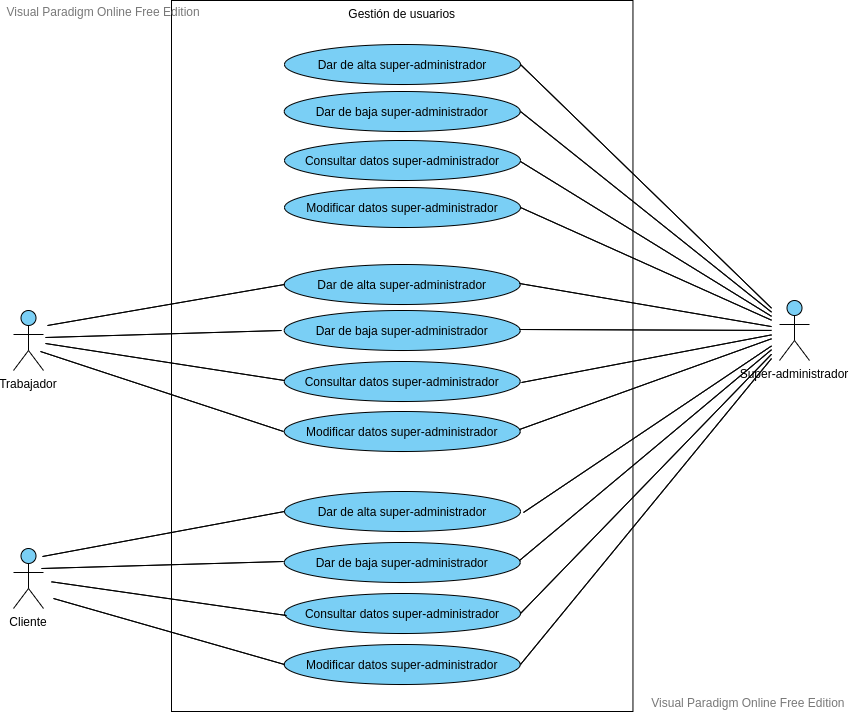
\includegraphics[width=0.9\textwidth]{images/Gestion_Usuarios.png}
    \caption{Diagrama de caso de uso - Gestión de usuarios}
    \label{CU1}
\end{figure}

\begin{figure}[H]
    \centering
    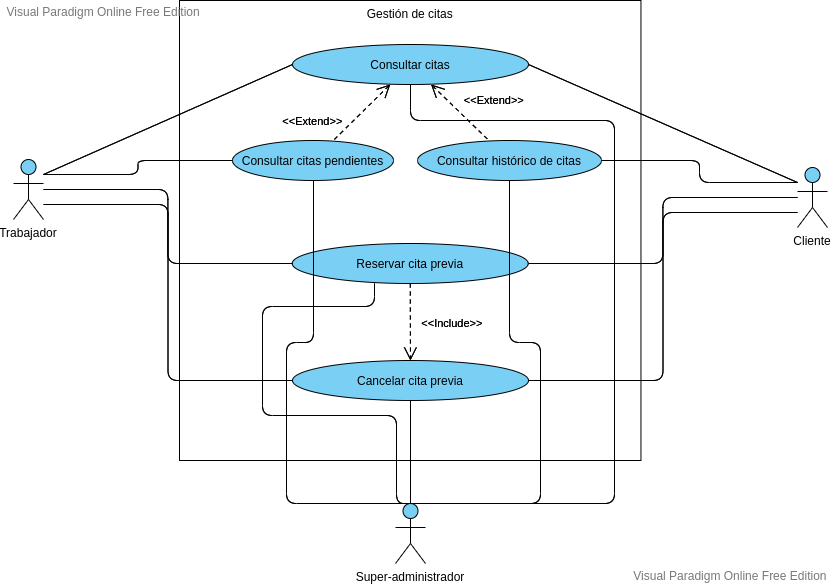
\includegraphics[width=0.9\textwidth]{images/Gestion_Citas.png}
    \caption{Diagrama de caso de uso - Gestión de citas}
    \label{CU1}
\end{figure}

\begin{figure}[H]
    \centering
    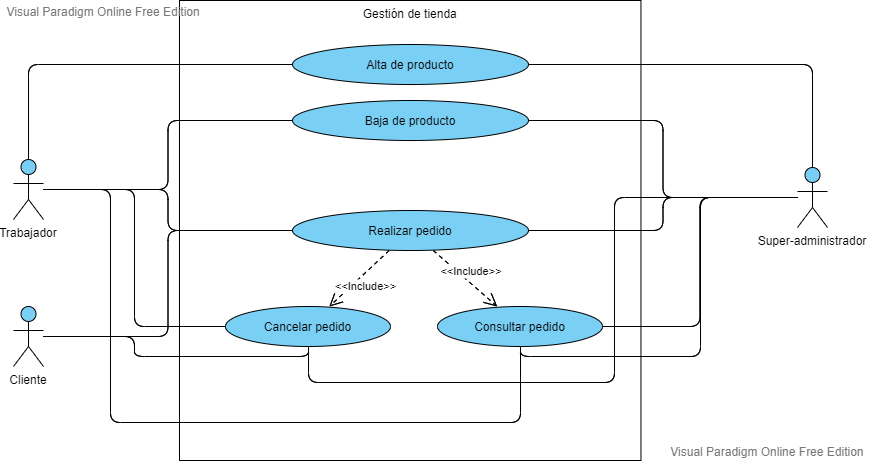
\includegraphics[width=0.9\textwidth]{images/Gestion_Tienda.png}
    \caption{Diagrama de caso de uso - Gestión de tienda}
    \label{CU1}
\end{figure}

\subsection{Descripción de los casos de uso}

En las siguientes tablas se detallan los casos de uso definidos en el apartado anterior. Podemos ver información sobre
los actores que interactuan en ella, el tipo, los requisitos funcionales incluidos, las precondiciones y
poscondiciones relativas a este y el propósito que cumple, además de un breve resumen que describe a un más alto
nivel lo que proporciona el caso de uso.

Los diferentes tipos de casos de uso son:

\begin{itemize}
    \item Según su importancia:
    \begin{itemize}
        \item Primarios: Procesos comunes más importantes.
        \item Secundarios: Procesos menores o raros.
        \item Opcionales: Procesos que pueden no abordarse.
    \end{itemize}

    \item Según el nivel de detalle
    \begin{itemize}
        \item Alto nivel: Descripción general del procesamiento.
        \item Extendidos: Descripción de la secuencia de acción completa entre actores y sistema.
    \end{itemize}

    \item Según el nivel de abstracción
    \begin{itemize}
        \item Esencial: Expresado de forma abstracta, contiene poca tecnología y pocos detalles de diseño.
        \item Real: Expresado en base al diseño actual, en el que aparecen relaciones con la interfaz de usuario.
    \end{itemize}
\end{itemize}

% SUPER-ADMINISTRADOR

\begin{table}[H]
\begin{tabular}{lll}
\hline
\rowcolor[HTML]{EFEFEF}
\multicolumn{1}{|l|}{\cellcolor[HTML]{EFEFEF}\textbf{Caso de uso}} & \multicolumn{1}{l|}{\cellcolor[HTML]{EFEFEF}
    Dar de alta super-administrador
} & \multicolumn{1}{l|}{\cellcolor[HTML]{EFEFEF}
    CU-1
} \\ \hline
\multicolumn{1}{|l|}{\textbf{Actores}} & \multicolumn{2}{l|}{
    Super-administrador
} \\ \hline
\multicolumn{1}{|l|}{\textbf{Tipo}} & \multicolumn{2}{l|}{
    Primario, básico y esencial
} \\ \hline
\multicolumn{1}{|l|}{\textbf{Referencias}} & \multicolumn{2}{l|}{
    RF-1.1
} \\ \hline
\multicolumn{1}{|l|}{\textbf{Precondición}} & \multicolumn{2}{l|}{\begin{tabular}[c]{@{}l@{}}
    Debe existir previamente un super-administrador que pueda \\ llevar a cabo esta función. Si no hay ninguno \\
    deberá añadirse por base de datos
\end{tabular}} \\ \hline
\multicolumn{1}{|l|}{\textbf{Poscondición}} & \multicolumn{2}{l|}{
    El super-administrador quedará registrado en el sistema
} \\ \hline
\multicolumn{3}{l}{} \\ \hline
\rowcolor[HTML]{EFEFEF}
\multicolumn{3}{|l|}{\cellcolor[HTML]{EFEFEF}\textbf{Propósito}} \\ \hline
\multicolumn{3}{|l|}{
    Dar de alta un nuevo super-administrador en el sistema
} \\ \hline
\multicolumn{3}{l}{} \\ \hline
\rowcolor[HTML]{EFEFEF}
\multicolumn{3}{|l|}{\cellcolor[HTML]{EFEFEF}\textbf{Resumen}} \\ \hline
\multicolumn{3}{|l|}{\begin{tabular}[c]{@{}l@{}}
    Se darán de alta usuarios con rol super-administrador, los cuales podrán \\ encargarse de la supervisión
    del sistema
\end{tabular}} \\ \hline
\end{tabular}
\end{table}

\begin{table}[H]
\begin{tabular}{lll}
\hline
\rowcolor[HTML]{EFEFEF}
\multicolumn{1}{|l|}{\cellcolor[HTML]{EFEFEF}\textbf{Caso de uso}} & \multicolumn{1}{l|}{\cellcolor[HTML]{EFEFEF}
    Dar de baja super-administrador
} & \multicolumn{1}{l|}{\cellcolor[HTML]{EFEFEF}
    CU-2
} \\ \hline
\multicolumn{1}{|l|}{\textbf{Actores}} & \multicolumn{2}{l|}{
    Super-administrador
} \\ \hline
\multicolumn{1}{|l|}{\textbf{Tipo}} & \multicolumn{2}{l|}{
    Primario, básico y esencial
} \\ \hline
\multicolumn{1}{|l|}{\textbf{Referencias}} & \multicolumn{2}{l|}{
    RF-1.2
} \\ \hline
\multicolumn{1}{|l|}{\textbf{Precondición}} & \multicolumn{2}{l|}{\begin{tabular}[c]{@{}l@{}}
    Debe existir previamente el super-administrador al que \\
    se quiera realizar la baja
\end{tabular}} \\ \hline
\multicolumn{1}{|l|}{\textbf{Poscondición}} & \multicolumn{2}{l|}{
    El super-administrador quedará eliminado del sistema
} \\ \hline
\multicolumn{3}{l}{} \\ \hline
\rowcolor[HTML]{EFEFEF}
\multicolumn{3}{|l|}{\cellcolor[HTML]{EFEFEF}\textbf{Propósito}} \\ \hline
\multicolumn{3}{|l|}{
    Dar de baja a un super-administrador del sistema
} \\ \hline
\multicolumn{3}{l}{} \\ \hline
\rowcolor[HTML]{EFEFEF}
\multicolumn{3}{|l|}{\cellcolor[HTML]{EFEFEF}\textbf{Resumen}} \\ \hline
\multicolumn{3}{|l|}{\begin{tabular}[c]{@{}l@{}}
    Se darán de baja a usuarios con rol super-administrador, eliminando \\
    su información de la base de datos del sistema
\end{tabular}} \\ \hline
\end{tabular}
\end{table}

\begin{table}[H]
\begin{tabular}{lll}
\hline
\rowcolor[HTML]{EFEFEF}
\multicolumn{1}{|l|}{\cellcolor[HTML]{EFEFEF}\textbf{Caso de uso}} & \multicolumn{1}{l|}{\cellcolor[HTML]{EFEFEF}
    Consultar datos del super-administrador
} & \multicolumn{1}{l|}{\cellcolor[HTML]{EFEFEF}
    CU-3
} \\ \hline
\multicolumn{1}{|l|}{\textbf{Actores}} & \multicolumn{2}{l|}{
    Super-administrador
} \\ \hline
\multicolumn{1}{|l|}{\textbf{Tipo}} & \multicolumn{2}{l|}{
    Primario, básico y esencial
} \\ \hline
\multicolumn{1}{|l|}{\textbf{Referencias}} & \multicolumn{2}{l|}{
    RF-1.3
} \\ \hline
\multicolumn{1}{|l|}{\textbf{Precondición}} & \multicolumn{2}{l|}{\begin{tabular}[c]{@{}l@{}}
    Debe existir previamente el super-administrador para \\
    poder consultar sus datos
\end{tabular}} \\ \hline
\multicolumn{1}{|l|}{\textbf{Poscondición}} & \multicolumn{2}{l|}{
    El super-administrador no sufrirá modificaciones
} \\ \hline
\multicolumn{3}{l}{} \\ \hline
\rowcolor[HTML]{EFEFEF}
\multicolumn{3}{|l|}{\cellcolor[HTML]{EFEFEF}\textbf{Propósito}} \\ \hline
\multicolumn{3}{|l|}{
    Consultar los datos personales como usuario super-administrador del sistema
} \\ \hline
\multicolumn{3}{l}{} \\ \hline
\rowcolor[HTML]{EFEFEF}
\multicolumn{3}{|l|}{\cellcolor[HTML]{EFEFEF}\textbf{Resumen}} \\ \hline
\multicolumn{3}{|l|}{\begin{tabular}[c]{@{}l@{}}
    Se podrá consultar los datos personales como usuario \\
    con rol super-administrador del sistema
\end{tabular}} \\ \hline
\end{tabular}
\end{table}

\begin{table}[H]
\begin{tabular}{lll}
\hline
\rowcolor[HTML]{EFEFEF}
\multicolumn{1}{|l|}{\cellcolor[HTML]{EFEFEF}\textbf{Caso de uso}} & \multicolumn{1}{l|}{\cellcolor[HTML]{EFEFEF}
    Modificar datos del super-administrador
} & \multicolumn{1}{l|}{\cellcolor[HTML]{EFEFEF}
    CU-4
} \\ \hline
\multicolumn{1}{|l|}{\textbf{Actores}} & \multicolumn{2}{l|}{
    Super-administrador
} \\ \hline
\multicolumn{1}{|l|}{\textbf{Tipo}} & \multicolumn{2}{l|}{
    Primario, básico y esencial
} \\ \hline
\multicolumn{1}{|l|}{\textbf{Referencias}} & \multicolumn{2}{l|}{
    RF-1.4
} \\ \hline
\multicolumn{1}{|l|}{\textbf{Precondición}} & \multicolumn{2}{l|}{\begin{tabular}[c]{@{}l@{}}
    Debe existir previamente el super-administrador para \\
    poder modificar sus datos personales
\end{tabular}} \\ \hline
\multicolumn{1}{|l|}{\textbf{Poscondición}} & \multicolumn{2}{l|}{
    Los datos del super-administrador sufrirán modificaciones
} \\ \hline
\multicolumn{3}{l}{} \\ \hline
\rowcolor[HTML]{EFEFEF}
\multicolumn{3}{|l|}{\cellcolor[HTML]{EFEFEF}\textbf{Propósito}} \\ \hline
\multicolumn{3}{|l|}{
    Modificar los datos personales como usuario super-administrador del sistema
} \\ \hline
\multicolumn{3}{l}{} \\ \hline
\rowcolor[HTML]{EFEFEF}
\multicolumn{3}{|l|}{\cellcolor[HTML]{EFEFEF}\textbf{Resumen}} \\ \hline
\multicolumn{3}{|l|}{\begin{tabular}[c]{@{}l@{}}
    Se podrán modificar los datos personales como usuario \\
    con rol super-administrador del sistema
\end{tabular}} \\ \hline
\end{tabular}
\end{table}

% TRABAJADORES

\begin{table}[H]
\begin{tabular}{lll}
\hline
\rowcolor[HTML]{EFEFEF}
\multicolumn{1}{|l|}{\cellcolor[HTML]{EFEFEF}\textbf{Caso de uso}} & \multicolumn{1}{l|}{\cellcolor[HTML]{EFEFEF}
    Dar de alta trabajador
} & \multicolumn{1}{l|}{\cellcolor[HTML]{EFEFEF}
    CU-5
} \\ \hline
\multicolumn{1}{|l|}{\textbf{Actores}} & \multicolumn{2}{l|}{
    Super-administrador y trabajador
} \\ \hline
\multicolumn{1}{|l|}{\textbf{Tipo}} & \multicolumn{2}{l|}{
    Primario, básico y esencial
} \\ \hline
\multicolumn{1}{|l|}{\textbf{Referencias}} & \multicolumn{2}{l|}{
    RF-2.1
} \\ \hline
\multicolumn{1}{|l|}{\textbf{Precondición}} & \multicolumn{2}{l|}{\begin{tabular}[c]{@{}l@{}}
    Debe existir previamente un super-administrador o \\
    un trabajador del negocio que pueda llevar a cabo \\
    esta función. Si no hay ninguno deberá añadirse \\
    por base de datos
\end{tabular}} \\ \hline
\multicolumn{1}{|l|}{\textbf{Poscondición}} & \multicolumn{2}{l|}{
    El trabajador quedará registrado en el sistema
} \\ \hline
\multicolumn{3}{l}{} \\ \hline
\rowcolor[HTML]{EFEFEF}
\multicolumn{3}{|l|}{\cellcolor[HTML]{EFEFEF}\textbf{Propósito}} \\ \hline
\multicolumn{3}{|l|}{
    Dar de alta un nuevo trabajador en el negocio
} \\ \hline
\multicolumn{3}{l}{} \\ \hline
\rowcolor[HTML]{EFEFEF}
\multicolumn{3}{|l|}{\cellcolor[HTML]{EFEFEF}\textbf{Resumen}} \\ \hline
\multicolumn{3}{|l|}{\begin{tabular}[c]{@{}l@{}}
    Se darán de alta usuarios con rol trabajador, los cuales podrán \\
    encargarse de la supervisión del negocio y atender citas
\end{tabular}} \\ \hline
\end{tabular}
\end{table}

\begin{table}[H]
\begin{tabular}{lll}
\hline
\rowcolor[HTML]{EFEFEF}
\multicolumn{1}{|l|}{\cellcolor[HTML]{EFEFEF}\textbf{Caso de uso}} & \multicolumn{1}{l|}{\cellcolor[HTML]{EFEFEF}
    Dar de baja trabajador
} & \multicolumn{1}{l|}{\cellcolor[HTML]{EFEFEF}
    CU-6
} \\ \hline
\multicolumn{1}{|l|}{\textbf{Actores}} & \multicolumn{2}{l|}{
    Super-administrador y trabajador
} \\ \hline
\multicolumn{1}{|l|}{\textbf{Tipo}} & \multicolumn{2}{l|}{
    Primario, básico y esencial
} \\ \hline
\multicolumn{1}{|l|}{\textbf{Referencias}} & \multicolumn{2}{l|}{
    RF-2.2
} \\ \hline
\multicolumn{1}{|l|}{\textbf{Precondición}} & \multicolumn{2}{l|}{\begin{tabular}[c]{@{}l@{}}
    Debe existir previamente el trabajador al que \\
    se quiera realizar la baja
\end{tabular}} \\ \hline
\multicolumn{1}{|l|}{\textbf{Poscondición}} & \multicolumn{2}{l|}{
    El trabajador quedará eliminado del sistema
} \\ \hline
\multicolumn{3}{l}{} \\ \hline
\rowcolor[HTML]{EFEFEF}
\multicolumn{3}{|l|}{\cellcolor[HTML]{EFEFEF}\textbf{Propósito}} \\ \hline
\multicolumn{3}{|l|}{
    Dar de baja a un trabajador del sistema
} \\ \hline
\multicolumn{3}{l}{} \\ \hline
\rowcolor[HTML]{EFEFEF}
\multicolumn{3}{|l|}{\cellcolor[HTML]{EFEFEF}\textbf{Resumen}} \\ \hline
\multicolumn{3}{|l|}{\begin{tabular}[c]{@{}l@{}}
    Se darán de baja a usuarios con rol trabajador, eliminando \\
    su información de la base de datos del sistema
\end{tabular}} \\ \hline
\end{tabular}
\end{table}

\begin{table}[H]
\begin{tabular}{lll}
\hline
\rowcolor[HTML]{EFEFEF}
\multicolumn{1}{|l|}{\cellcolor[HTML]{EFEFEF}\textbf{Caso de uso}} & \multicolumn{1}{l|}{\cellcolor[HTML]{EFEFEF}
    Consultar datos del trabajador
} & \multicolumn{1}{l|}{\cellcolor[HTML]{EFEFEF}
    CU-7
} \\ \hline
\multicolumn{1}{|l|}{\textbf{Actores}} & \multicolumn{2}{l|}{
    Super-administrador y trabajador
} \\ \hline
\multicolumn{1}{|l|}{\textbf{Tipo}} & \multicolumn{2}{l|}{
    Primario, básico y esencial
} \\ \hline
\multicolumn{1}{|l|}{\textbf{Referencias}} & \multicolumn{2}{l|}{
    RF-2.3
} \\ \hline
\multicolumn{1}{|l|}{\textbf{Precondición}} & \multicolumn{2}{l|}{\begin{tabular}[c]{@{}l@{}}
    Debe existir previamente el trabajador para \\
    poder consultar sus datos
\end{tabular}} \\ \hline
\multicolumn{1}{|l|}{\textbf{Poscondición}} & \multicolumn{2}{l|}{
    El trabajador no sufrirá modificaciones
} \\ \hline
\multicolumn{3}{l}{} \\ \hline
\rowcolor[HTML]{EFEFEF}
\multicolumn{3}{|l|}{\cellcolor[HTML]{EFEFEF}\textbf{Propósito}} \\ \hline
\multicolumn{3}{|l|}{\begin{tabular}[c]{@{}l@{}}{
    Consultar los datos personales como usuario trabajador del sistema \\
    de un negocio determinado
} \\ \hline
\end{tabular}} \\ \hline
\multicolumn{3}{l}{} \\ \hline
\rowcolor[HTML]{EFEFEF}
\multicolumn{3}{|l|}{\cellcolor[HTML]{EFEFEF}\textbf{Resumen}} \\ \hline
\multicolumn{3}{|l|}{\begin{tabular}[c]{@{}l@{}}
    Se podrá consultar los datos personales como usuario \\
    con rol trabajador del sistema de un negocio determinado
\end{tabular}} \\ \hline
\end{tabular}
\end{table}

\begin{table}[H]
\begin{tabular}{lll}
\hline
\rowcolor[HTML]{EFEFEF}
\multicolumn{1}{|l|}{\cellcolor[HTML]{EFEFEF}\textbf{Caso de uso}} & \multicolumn{1}{l|}{\cellcolor[HTML]{EFEFEF}
    Modificar datos del trabajador
} & \multicolumn{1}{l|}{\cellcolor[HTML]{EFEFEF}
    CU-8
} \\ \hline
\multicolumn{1}{|l|}{\textbf{Actores}} & \multicolumn{2}{l|}{
    Super-administrador y trabajador
} \\ \hline
\multicolumn{1}{|l|}{\textbf{Tipo}} & \multicolumn{2}{l|}{
    Primario, básico y esencial
} \\ \hline
\multicolumn{1}{|l|}{\textbf{Referencias}} & \multicolumn{2}{l|}{
    RF-2.4
} \\ \hline
\multicolumn{1}{|l|}{\textbf{Precondición}} & \multicolumn{2}{l|}{\begin{tabular}[c]{@{}l@{}}
    Debe existir previamente el trabajador para \\
    poder modificar sus datos personales
\end{tabular}} \\ \hline
\multicolumn{1}{|l|}{\textbf{Poscondición}} & \multicolumn{2}{l|}{
    Los datos del trabajador sufrirán modificaciones
} \\ \hline
\multicolumn{3}{l}{} \\ \hline
\rowcolor[HTML]{EFEFEF}
\multicolumn{3}{|l|}{\cellcolor[HTML]{EFEFEF}\textbf{Propósito}} \\ \hline
\multicolumn{3}{|l|}{\begin{tabular}[c]{@{}l@{}}{
    Modificar los datos personales como usuario trabajador del sistema \\
    de un negocio determinado
} \\ \hline
\end{tabular}} \\ \hline
\multicolumn{3}{l}{} \\ \hline
\rowcolor[HTML]{EFEFEF}
\multicolumn{3}{|l|}{\cellcolor[HTML]{EFEFEF}\textbf{Resumen}} \\ \hline
\multicolumn{3}{|l|}{\begin{tabular}[c]{@{}l@{}}
    Se podrán modificar los datos personales como usuario \\
    con rol trabajador del sistema de un negocio determinado
\end{tabular}} \\ \hline
\end{tabular}
\end{table}

% CLIENTES

\begin{table}[H]
\begin{tabular}{lll}
\hline
\rowcolor[HTML]{EFEFEF}
\multicolumn{1}{|l|}{\cellcolor[HTML]{EFEFEF}\textbf{Caso de uso}} & \multicolumn{1}{l|}{\cellcolor[HTML]{EFEFEF}
    Dar de alta cliente
} & \multicolumn{1}{l|}{\cellcolor[HTML]{EFEFEF}
    CU-9
} \\ \hline
\multicolumn{1}{|l|}{\textbf{Actores}} & \multicolumn{2}{l|}{
    Super-administrador, trabajador y cliente
} \\ \hline
\multicolumn{1}{|l|}{\textbf{Tipo}} & \multicolumn{2}{l|}{
    Primario, básico y esencial
} \\ \hline
\multicolumn{1}{|l|}{\textbf{Referencias}} & \multicolumn{2}{l|}{
    RF-3.1
} \\ \hline
\multicolumn{1}{|l|}{\textbf{Precondición}} & \multicolumn{2}{l|}{\begin{tabular}[c]{@{}l@{}}
    Un cliente puede darse de alta en un negocio sin \\
    precondiciones
\end{tabular}} \\ \hline
\multicolumn{1}{|l|}{\textbf{Poscondición}} & \multicolumn{2}{l|}{
    El cliente quedará registrado en el sistema
} \\ \hline
\multicolumn{3}{l}{} \\ \hline
\rowcolor[HTML]{EFEFEF}
\multicolumn{3}{|l|}{\cellcolor[HTML]{EFEFEF}\textbf{Propósito}} \\ \hline
\multicolumn{3}{|l|}{
    Dar de alta un nuevo cliente en el negocio
} \\ \hline
\multicolumn{3}{l}{} \\ \hline
\rowcolor[HTML]{EFEFEF}
\multicolumn{3}{|l|}{\cellcolor[HTML]{EFEFEF}\textbf{Resumen}} \\ \hline
\multicolumn{3}{|l|}{\begin{tabular}[c]{@{}l@{}}
    Se darán de alta usuarios con rol cliente, los cuales podrán \\
    realizar acciones en el negocio determinado
\end{tabular}} \\ \hline
\end{tabular}
\end{table}

\begin{table}[H]
\begin{tabular}{lll}
\hline
\rowcolor[HTML]{EFEFEF}
\multicolumn{1}{|l|}{\cellcolor[HTML]{EFEFEF}\textbf{Caso de uso}} & \multicolumn{1}{l|}{\cellcolor[HTML]{EFEFEF}
    Dar de baja cliente
} & \multicolumn{1}{l|}{\cellcolor[HTML]{EFEFEF}
    CU-10
} \\ \hline
\multicolumn{1}{|l|}{\textbf{Actores}} & \multicolumn{2}{l|}{
    Super-administrador, trabajador y cliente
} \\ \hline
\multicolumn{1}{|l|}{\textbf{Tipo}} & \multicolumn{2}{l|}{
    Primario, básico y esencial
} \\ \hline
\multicolumn{1}{|l|}{\textbf{Referencias}} & \multicolumn{2}{l|}{
    RF-3.2
} \\ \hline
\multicolumn{1}{|l|}{\textbf{Precondición}} & \multicolumn{2}{l|}{\begin{tabular}[c]{@{}l@{}}
    Debe existir previamente el cliente al que \\
    se quiera realizar la baja
\end{tabular}} \\ \hline
\multicolumn{1}{|l|}{\textbf{Poscondición}} & \multicolumn{2}{l|}{
    El cliente quedará eliminado del sistema
} \\ \hline
\multicolumn{3}{l}{} \\ \hline
\rowcolor[HTML]{EFEFEF}
\multicolumn{3}{|l|}{\cellcolor[HTML]{EFEFEF}\textbf{Propósito}} \\ \hline
\multicolumn{3}{|l|}{
    Dar de baja a un cliente del sistema
} \\ \hline
\multicolumn{3}{l}{} \\ \hline
\rowcolor[HTML]{EFEFEF}
\multicolumn{3}{|l|}{\cellcolor[HTML]{EFEFEF}\textbf{Resumen}} \\ \hline
\multicolumn{3}{|l|}{\begin{tabular}[c]{@{}l@{}}
    Se darán de baja a usuarios con rol cliente, eliminando \\
    su información de la base de datos del sistema
\end{tabular}} \\ \hline
\end{tabular}
\end{table}

\begin{table}[H]
\begin{tabular}{lll}
\hline
\rowcolor[HTML]{EFEFEF}
\multicolumn{1}{|l|}{\cellcolor[HTML]{EFEFEF}\textbf{Caso de uso}} & \multicolumn{1}{l|}{\cellcolor[HTML]{EFEFEF}
    Consultar datos del cliente
} & \multicolumn{1}{l|}{\cellcolor[HTML]{EFEFEF}
    CU-11
} \\ \hline
\multicolumn{1}{|l|}{\textbf{Actores}} & \multicolumn{2}{l|}{
    Super-administrador, trabajador y cliente
} \\ \hline
\multicolumn{1}{|l|}{\textbf{Tipo}} & \multicolumn{2}{l|}{
    Primario, básico y esencial
} \\ \hline
\multicolumn{1}{|l|}{\textbf{Referencias}} & \multicolumn{2}{l|}{
    RF-3.3
} \\ \hline
\multicolumn{1}{|l|}{\textbf{Precondición}} & \multicolumn{2}{l|}{\begin{tabular}[c]{@{}l@{}}
    Debe existir previamente el cliente para \\
    poder consultar sus datos
\end{tabular}} \\ \hline
\multicolumn{1}{|l|}{\textbf{Poscondición}} & \multicolumn{2}{l|}{
    El cliente no sufrirá modificaciones
} \\ \hline
\multicolumn{3}{l}{} \\ \hline
\rowcolor[HTML]{EFEFEF}
\multicolumn{3}{|l|}{\cellcolor[HTML]{EFEFEF}\textbf{Propósito}} \\ \hline
\multicolumn{3}{|l|}{\begin{tabular}[c]{@{}l@{}}{
    Consultar los datos personales como usuario cliente del sistema \\
    de un negocio determinado
} \\ \hline
\end{tabular}} \\ \hline
\multicolumn{3}{l}{} \\ \hline
\rowcolor[HTML]{EFEFEF}
\multicolumn{3}{|l|}{\cellcolor[HTML]{EFEFEF}\textbf{Resumen}} \\ \hline
\multicolumn{3}{|l|}{\begin{tabular}[c]{@{}l@{}}
    Se podrá consultar los datos personales como usuario \\
    con rol cliente del sistema de un negocio determinado
\end{tabular}} \\ \hline
\end{tabular}
\end{table}

\begin{table}[H]
\begin{tabular}{lll}
\hline
\rowcolor[HTML]{EFEFEF}
\multicolumn{1}{|l|}{\cellcolor[HTML]{EFEFEF}\textbf{Caso de uso}} & \multicolumn{1}{l|}{\cellcolor[HTML]{EFEFEF}
    Modificar datos del cliente
} & \multicolumn{1}{l|}{\cellcolor[HTML]{EFEFEF}
    CU-12
} \\ \hline
\multicolumn{1}{|l|}{\textbf{Actores}} & \multicolumn{2}{l|}{
    Cliente
} \\ \hline
\multicolumn{1}{|l|}{\textbf{Tipo}} & \multicolumn{2}{l|}{
    Primario, básico y esencial
} \\ \hline
\multicolumn{1}{|l|}{\textbf{Referencias}} & \multicolumn{2}{l|}{
    RF-3.4
} \\ \hline
\multicolumn{1}{|l|}{\textbf{Precondición}} & \multicolumn{2}{l|}{\begin{tabular}[c]{@{}l@{}}
    Debe existir previamente el cliente para \\
    poder modificar sus datos personales
\end{tabular}} \\ \hline
\multicolumn{1}{|l|}{\textbf{Poscondición}} & \multicolumn{2}{l|}{
    Los datos del cliente sufrirán modificaciones
} \\ \hline
\multicolumn{3}{l}{} \\ \hline
\rowcolor[HTML]{EFEFEF}
\multicolumn{3}{|l|}{\cellcolor[HTML]{EFEFEF}\textbf{Propósito}} \\ \hline
\multicolumn{3}{|l|}{\begin{tabular}[c]{@{}l@{}}{
    Modificar los datos personales como usuario cliente del sistema \\
    de un negocio determinado
} \\ \hline
\end{tabular}} \\ \hline
\multicolumn{3}{l}{} \\ \hline
\rowcolor[HTML]{EFEFEF}
\multicolumn{3}{|l|}{\cellcolor[HTML]{EFEFEF}\textbf{Resumen}} \\ \hline
\multicolumn{3}{|l|}{\begin{tabular}[c]{@{}l@{}}
    Se podrán modificar los datos personales como usuario \\
    con rol cliente del sistema de un negocio determinado
\end{tabular}} \\ \hline
\end{tabular}
\end{table}

% CITAS

\begin{table}[H]
\begin{tabular}{lll}
\hline
\rowcolor[HTML]{EFEFEF}
\multicolumn{1}{|l|}{\cellcolor[HTML]{EFEFEF}\textbf{Caso de uso}} & \multicolumn{1}{l|}{\cellcolor[HTML]{EFEFEF}
    Consultar citas
} & \multicolumn{1}{l|}{\cellcolor[HTML]{EFEFEF}
    CU-13
} \\ \hline
\multicolumn{1}{|l|}{\textbf{Actores}} & \multicolumn{2}{l|}{
    Trabajador y cliente
} \\ \hline
\multicolumn{1}{|l|}{\textbf{Tipo}} & \multicolumn{2}{l|}{
    Primario, básico y esencial
} \\ \hline
\multicolumn{1}{|l|}{\textbf{Referencias}} & \multicolumn{2}{l|}{
    RF-2.5, RF-3.5
} \\ \hline
\multicolumn{1}{|l|}{\textbf{Precondición}} & \multicolumn{2}{l|}{\begin{tabular}[c]{@{}l@{}}
    Debe existir previamente el usuario para \\
    consultar sus citas
\end{tabular}} \\ \hline
\multicolumn{1}{|l|}{\textbf{Poscondición}} & \multicolumn{2}{l|}{
    Las citas del usuario no sufrirán modificaciones
} \\ \hline
\multicolumn{3}{l}{} \\ \hline
\rowcolor[HTML]{EFEFEF}
\multicolumn{3}{|l|}{\cellcolor[HTML]{EFEFEF}\textbf{Propósito}} \\ \hline
\multicolumn{3}{|l|}{\begin{tabular}[c]{@{}l@{}}{
    Consultar las citas de los usuarios de un negocio determinado
} \\ \hline
\end{tabular}} \\ \hline
\multicolumn{3}{l}{} \\ \hline
\rowcolor[HTML]{EFEFEF}
\multicolumn{3}{|l|}{\cellcolor[HTML]{EFEFEF}\textbf{Resumen}} \\ \hline
\multicolumn{3}{|l|}{\begin{tabular}[c]{@{}l@{}}
    Un usuario podrá consultar sus citas asignadas, ya \\
    sea un trabajador para ver sus citas atendidas y \\
    por atender, o un cliente para ver sus citas reservadas
\end{tabular}} \\ \hline
\end{tabular}
\end{table}

\begin{table}[H]
\begin{tabular}{lll}
\hline
\rowcolor[HTML]{EFEFEF}
\multicolumn{1}{|l|}{\cellcolor[HTML]{EFEFEF}\textbf{Caso de uso}} & \multicolumn{1}{l|}{\cellcolor[HTML]{EFEFEF}
    Consultar citas pendientes
} & \multicolumn{1}{l|}{\cellcolor[HTML]{EFEFEF}
    CU-14
} \\ \hline
\multicolumn{1}{|l|}{\textbf{Actores}} & \multicolumn{2}{l|}{
    Trabajador y cliente
} \\ \hline
\multicolumn{1}{|l|}{\textbf{Tipo}} & \multicolumn{2}{l|}{
    Primario, básico y esencial
} \\ \hline
\multicolumn{1}{|l|}{\textbf{Referencias}} & \multicolumn{2}{l|}{
    RF-2.5, RF-3.5
} \\ \hline
\multicolumn{1}{|l|}{\textbf{Precondición}} & \multicolumn{2}{l|}{\begin{tabular}[c]{@{}l@{}}
    Debe existir previamente el usuario para \\
    consultar sus citas pendientes
\end{tabular}} \\ \hline
\multicolumn{1}{|l|}{\textbf{Poscondición}} & \multicolumn{2}{l|}{
    Las citas del usuario no sufrirán modificaciones
} \\ \hline
\multicolumn{3}{l}{} \\ \hline
\rowcolor[HTML]{EFEFEF}
\multicolumn{3}{|l|}{\cellcolor[HTML]{EFEFEF}\textbf{Propósito}} \\ \hline
\multicolumn{3}{|l|}{\begin{tabular}[c]{@{}l@{}}{
    Consultar las citas pendientes de los usuarios de un \\
    negocio determinado
} \\ \hline
\end{tabular}} \\ \hline
\multicolumn{3}{l}{} \\ \hline
\rowcolor[HTML]{EFEFEF}
\multicolumn{3}{|l|}{\cellcolor[HTML]{EFEFEF}\textbf{Resumen}} \\ \hline
\multicolumn{3}{|l|}{\begin{tabular}[c]{@{}l@{}}
    Un usuario podrá consultar sus citas pendientes, ya \\
    sea un trabajador para ver sus citas a atender, \\
    o un cliente para ver sus citas reservadas pendientes
\end{tabular}} \\ \hline
\end{tabular}
\end{table}

\begin{table}[H]
\begin{tabular}{lll}
\hline
\rowcolor[HTML]{EFEFEF}
\multicolumn{1}{|l|}{\cellcolor[HTML]{EFEFEF}\textbf{Caso de uso}} & \multicolumn{1}{l|}{\cellcolor[HTML]{EFEFEF}
    Consultar histórico de citas
} & \multicolumn{1}{l|}{\cellcolor[HTML]{EFEFEF}
    CU-15
} \\ \hline
\multicolumn{1}{|l|}{\textbf{Actores}} & \multicolumn{2}{l|}{
    Trabajador y cliente
} \\ \hline
\multicolumn{1}{|l|}{\textbf{Tipo}} & \multicolumn{2}{l|}{
    Primario, básico y esencial
} \\ \hline
\multicolumn{1}{|l|}{\textbf{Referencias}} & \multicolumn{2}{l|}{
    RF-2.5, RF-3.5
} \\ \hline
\multicolumn{1}{|l|}{\textbf{Precondición}} & \multicolumn{2}{l|}{\begin{tabular}[c]{@{}l@{}}
    Debe existir previamente el usuario para \\
    consultar su histórico de citas
\end{tabular}} \\ \hline
\multicolumn{1}{|l|}{\textbf{Poscondición}} & \multicolumn{2}{l|}{
    Las citas del usuario no sufrirán modificaciones
} \\ \hline
\multicolumn{3}{l}{} \\ \hline
\rowcolor[HTML]{EFEFEF}
\multicolumn{3}{|l|}{\cellcolor[HTML]{EFEFEF}\textbf{Propósito}} \\ \hline
\multicolumn{3}{|l|}{\begin{tabular}[c]{@{}l@{}}{
    Consultar el histórico de citas de los usuarios de un \\
    negocio determinado
} \\ \hline
\end{tabular}} \\ \hline
\multicolumn{3}{l}{} \\ \hline
\rowcolor[HTML]{EFEFEF}
\multicolumn{3}{|l|}{\cellcolor[HTML]{EFEFEF}\textbf{Resumen}} \\ \hline
\multicolumn{3}{|l|}{\begin{tabular}[c]{@{}l@{}}
    Un usuario podrá consultar su histórico de citas, ya \\
    sea un trabajador o un cliente para ver sus citas \\
    registradas
\end{tabular}} \\ \hline
\end{tabular}
\end{table}

\begin{table}[H]
\begin{tabular}{lll}
\hline
\rowcolor[HTML]{EFEFEF}
\multicolumn{1}{|l|}{\cellcolor[HTML]{EFEFEF}\textbf{Caso de uso}} & \multicolumn{1}{l|}{\cellcolor[HTML]{EFEFEF}
    Reservar cita previa
} & \multicolumn{1}{l|}{\cellcolor[HTML]{EFEFEF}
    CU-16
} \\ \hline
\multicolumn{1}{|l|}{\textbf{Actores}} & \multicolumn{2}{l|}{
    Trabajador y cliente
} \\ \hline
\multicolumn{1}{|l|}{\textbf{Tipo}} & \multicolumn{2}{l|}{
    Primario, básico y esencial
} \\ \hline
\multicolumn{1}{|l|}{\textbf{Referencias}} & \multicolumn{2}{l|}{
    RF-4.1, RF-4.3
} \\ \hline
\multicolumn{1}{|l|}{\textbf{Precondición}} & \multicolumn{2}{l|}{\begin{tabular}[c]{@{}l@{}}
    Debe existir previamente el usuario del \\
    cliente y el trabajador para \\
    reservar una cita previa
\end{tabular}} \\ \hline
\multicolumn{1}{|l|}{\textbf{Poscondición}} & \multicolumn{2}{l|}{
    Se reserverá una cita para un cliente
} \\ \hline
\multicolumn{3}{l}{} \\ \hline
\rowcolor[HTML]{EFEFEF}
\multicolumn{3}{|l|}{\cellcolor[HTML]{EFEFEF}\textbf{Propósito}} \\ \hline
\multicolumn{3}{|l|}{\begin{tabular}[c]{@{}l@{}}{
    Reservar una cita para un cliente y trabajador determinado
} \\ \hline
\end{tabular}} \\ \hline
\multicolumn{3}{l}{} \\ \hline
\rowcolor[HTML]{EFEFEF}
\multicolumn{3}{|l|}{\cellcolor[HTML]{EFEFEF}\textbf{Resumen}} \\ \hline
\multicolumn{3}{|l|}{\begin{tabular}[c]{@{}l@{}}
    Un usuario podrá reservar una cita previa disponible con \\
    un trabajador determinado. De la misma forma un trabajador \\
    disponible podrá reservar para un cliente existente que \\
    aún no disponga de cita reservada
\end{tabular}} \\ \hline
\end{tabular}
\end{table}

\begin{table}[H]
\begin{tabular}{lll}
\hline
\rowcolor[HTML]{EFEFEF}
\multicolumn{1}{|l|}{\cellcolor[HTML]{EFEFEF}\textbf{Caso de uso}} & \multicolumn{1}{l|}{\cellcolor[HTML]{EFEFEF}
    Cancelar cita previa
} & \multicolumn{1}{l|}{\cellcolor[HTML]{EFEFEF}
    CU-17
} \\ \hline
\multicolumn{1}{|l|}{\textbf{Actores}} & \multicolumn{2}{l|}{
    Trabajador y cliente
} \\ \hline
\multicolumn{1}{|l|}{\textbf{Tipo}} & \multicolumn{2}{l|}{
    Primario, básico y esencial
} \\ \hline
\multicolumn{1}{|l|}{\textbf{Referencias}} & \multicolumn{2}{l|}{
    RF-4.2, RF-4.4
} \\ \hline
\multicolumn{1}{|l|}{\textbf{Precondición}} & \multicolumn{2}{l|}{\begin{tabular}[c]{@{}l@{}}
    Debe existir previamente el usuario con \\
    la cita reservada en estado pendiente
\end{tabular}} \\ \hline
\multicolumn{1}{|l|}{\textbf{Poscondición}} & \multicolumn{2}{l|}{
    Se cancelará una cita para un cliente
} \\ \hline
\multicolumn{3}{l}{} \\ \hline
\rowcolor[HTML]{EFEFEF}
\multicolumn{3}{|l|}{\cellcolor[HTML]{EFEFEF}\textbf{Propósito}} \\ \hline
\multicolumn{3}{|l|}{\begin{tabular}[c]{@{}l@{}}{
    Cancelar una cita para un cliente determinado
} \\ \hline
\end{tabular}} \\ \hline
\multicolumn{3}{l}{} \\ \hline
\rowcolor[HTML]{EFEFEF}
\multicolumn{3}{|l|}{\cellcolor[HTML]{EFEFEF}\textbf{Resumen}} \\ \hline
\multicolumn{3}{|l|}{\begin{tabular}[c]{@{}l@{}}
    Un usuario podrá cancelar su cita previa pendiente.\\
    De la misma forma un trabajador podrá cancelar una\\
    cita a un cliente el cual se le había asignado.
\end{tabular}} \\ \hline
\end{tabular}
\end{table}

\begin{table}[H]
\begin{tabular}{lll}
\hline
\rowcolor[HTML]{EFEFEF}
\multicolumn{1}{|l|}{\cellcolor[HTML]{EFEFEF}\textbf{Caso de uso}} & \multicolumn{1}{l|}{\cellcolor[HTML]{EFEFEF}
    Alta de producto
} & \multicolumn{1}{l|}{\cellcolor[HTML]{EFEFEF}
    CU-18
} \\ \hline
\multicolumn{1}{|l|}{\textbf{Actores}} & \multicolumn{2}{l|}{
    Trabajador y super-administrador
} \\ \hline
\multicolumn{1}{|l|}{\textbf{Tipo}} & \multicolumn{2}{l|}{
    Primario, básico y esencial
} \\ \hline
\multicolumn{1}{|l|}{\textbf{Referencias}} & \multicolumn{2}{l|}{
    RF-5.1
} \\ \hline
\multicolumn{1}{|l|}{\textbf{Precondición}} & \multicolumn{2}{l|}{\begin{tabular}[c]{@{}l@{}}
    El producto no debe exister ya en el sistema
\end{tabular}} \\ \hline
\multicolumn{1}{|l|}{\textbf{Poscondición}} & \multicolumn{2}{l|}{
    Se dará de alta un nuevo producto
} \\ \hline
\multicolumn{3}{l}{} \\ \hline
\rowcolor[HTML]{EFEFEF}
\multicolumn{3}{|l|}{\cellcolor[HTML]{EFEFEF}\textbf{Propósito}} \\ \hline
\multicolumn{3}{|l|}{\begin{tabular}[c]{@{}l@{}}{
    Dar de alta un nuevo producto para su venta
} \\ \hline
\end{tabular}} \\ \hline
\multicolumn{3}{l}{} \\ \hline
\rowcolor[HTML]{EFEFEF}
\multicolumn{3}{|l|}{\cellcolor[HTML]{EFEFEF}\textbf{Resumen}} \\ \hline
\multicolumn{3}{|l|}{\begin{tabular}[c]{@{}l@{}}
    Un trabajador o super-administrador del sistema \\
    podrá dar de alta un producto para su negocio \\
    determinado, estando este disponible para su venta \\
    online.
\end{tabular}} \\ \hline
\end{tabular}
\end{table}

\begin{table}[H]
\begin{tabular}{lll}
\hline
\rowcolor[HTML]{EFEFEF}
\multicolumn{1}{|l|}{\cellcolor[HTML]{EFEFEF}\textbf{Caso de uso}} & \multicolumn{1}{l|}{\cellcolor[HTML]{EFEFEF}
    Baja de producto
} & \multicolumn{1}{l|}{\cellcolor[HTML]{EFEFEF}
    CU-19
} \\ \hline
\multicolumn{1}{|l|}{\textbf{Actores}} & \multicolumn{2}{l|}{
    Trabajador y super-administrador
} \\ \hline
\multicolumn{1}{|l|}{\textbf{Tipo}} & \multicolumn{2}{l|}{
    Primario, básico y esencial
} \\ \hline
\multicolumn{1}{|l|}{\textbf{Referencias}} & \multicolumn{2}{l|}{
    RF-5.2
} \\ \hline
\multicolumn{1}{|l|}{\textbf{Precondición}} & \multicolumn{2}{l|}{\begin{tabular}[c]{@{}l@{}}
    El producto debe exister en el sistema
\end{tabular}} \\ \hline
\multicolumn{1}{|l|}{\textbf{Poscondición}} & \multicolumn{2}{l|}{
    Se dará de baja un producto
} \\ \hline
\multicolumn{3}{l}{} \\ \hline
\rowcolor[HTML]{EFEFEF}
\multicolumn{3}{|l|}{\cellcolor[HTML]{EFEFEF}\textbf{Propósito}} \\ \hline
\multicolumn{3}{|l|}{\begin{tabular}[c]{@{}l@{}}{
    Dar de baja un producto para su venta
} \\ \hline
\end{tabular}} \\ \hline
\multicolumn{3}{l}{} \\ \hline
\rowcolor[HTML]{EFEFEF}
\multicolumn{3}{|l|}{\cellcolor[HTML]{EFEFEF}\textbf{Resumen}} \\ \hline
\multicolumn{3}{|l|}{\begin{tabular}[c]{@{}l@{}}
    Un trabajador o super-administrador del sistema \\
    podrá dar de baja un producto para su negocio \\
    determinado, eliminando la disponible para su venta \\
    online.
\end{tabular}} \\ \hline
\end{tabular}
\end{table}

\begin{table}[H]
\begin{tabular}{lll}
\hline
\rowcolor[HTML]{EFEFEF}
\multicolumn{1}{|l|}{\cellcolor[HTML]{EFEFEF}\textbf{Caso de uso}} & \multicolumn{1}{l|}{\cellcolor[HTML]{EFEFEF}
    Realizar pedido
} & \multicolumn{1}{l|}{\cellcolor[HTML]{EFEFEF}
    CU-20
} \\ \hline
\multicolumn{1}{|l|}{\textbf{Actores}} & \multicolumn{2}{l|}{
    Cliente
} \\ \hline
\multicolumn{1}{|l|}{\textbf{Tipo}} & \multicolumn{2}{l|}{
    Primario, básico y esencial
} \\ \hline
\multicolumn{1}{|l|}{\textbf{Referencias}} & \multicolumn{2}{l|}{
    RF-6.1
} \\ \hline
\multicolumn{1}{|l|}{\textbf{Precondición}} & \multicolumn{2}{l|}{\begin{tabular}[c]{@{}l@{}}
    El pedido no puede tener cero productos
\end{tabular}} \\ \hline
\multicolumn{1}{|l|}{\textbf{Poscondición}} & \multicolumn{2}{1|}{
    Se reducirá el stock correspondiente
} \\ \hline
\multicolumn{3}{l}{} \\ \hline
\rowcolor[HTML]{EFEFEF}
\multicolumn{3}{|l|}{\cellcolor[HTML]{EFEFEF}\textbf{Propósito}} \\ \hline
\multicolumn{3}{|l|}{\begin{tabular}[c]{@{}l@{}}{
    Realizar un pedido de productos
} \\ \hline
\end{tabular}} \\ \hline
\multicolumn{3}{l}{} \\ \hline
\rowcolor[HTML]{EFEFEF}
\multicolumn{3}{|l|}{\cellcolor[HTML]{EFEFEF}\textbf{Resumen}} \\ \hline
\multicolumn{3}{|l|}{\begin{tabular}[c]{@{}l@{}}
    Un cliente podrá realizar un pedido de productos \\
    ofertados en la tienda online del negocio.
\end{tabular}} \\ \hline
\end{tabular}
\end{table}

\begin{table}[H]
\begin{tabular}{lll}
\hline
\rowcolor[HTML]{EFEFEF}
\multicolumn{1}{|l|}{\cellcolor[HTML]{EFEFEF}\textbf{Caso de uso}} & \multicolumn{1}{l|}{\cellcolor[HTML]{EFEFEF}
    Cancelación de pedido
} & \multicolumn{1}{l|}{\cellcolor[HTML]{EFEFEF}
    CU-21
} \\ \hline
\multicolumn{1}{|l|}{\textbf{Actores}} & \multicolumn{2}{l|}{
    Cliente
} \\ \hline
\multicolumn{1}{|l|}{\textbf{Tipo}} & \multicolumn{2}{l|}{
    Primario, básico y esencial
} \\ \hline
\multicolumn{1}{|l|}{\textbf{Referencias}} & \multicolumn{2}{l|}{
    RF-6.2
} \\ \hline
\multicolumn{1}{|l|}{\textbf{Precondición}} & \multicolumn{2}{l|}{\begin{tabular}[c]{@{}l@{}}
    Deberá existir un pedido en estado pendiente
\end{tabular}} \\ \hline
\multicolumn{1}{|l|}{\textbf{Poscondición}} & \multicolumn{2}{1|}{
    Se cancelará el pedido pendiente
} \\ \hline
\multicolumn{3}{l}{} \\ \hline
\rowcolor[HTML]{EFEFEF}
\multicolumn{3}{|l|}{\cellcolor[HTML]{EFEFEF}\textbf{Propósito}} \\ \hline
\multicolumn{3}{|l|}{\begin{tabular}[c]{@{}l@{}}{
    Cancelar un pedido pendiente
} \\ \hline
\end{tabular}} \\ \hline
\multicolumn{3}{l}{} \\ \hline
\rowcolor[HTML]{EFEFEF}
\multicolumn{3}{|l|}{\cellcolor[HTML]{EFEFEF}\textbf{Resumen}} \\ \hline
\multicolumn{3}{|l|}{\begin{tabular}[c]{@{}l@{}}
    Un cliente podrá cancelar un pedido que se encuentre \\
    en estado pendiente.
\end{tabular}} \\ \hline
\end{tabular}
\end{table}

\begin{table}[H]
\begin{tabular}{lll}
\hline
\rowcolor[HTML]{EFEFEF}
\multicolumn{1}{|l|}{\cellcolor[HTML]{EFEFEF}\textbf{Caso de uso}} & \multicolumn{1}{l|}{\cellcolor[HTML]{EFEFEF}
    Consultar de pedido
} & \multicolumn{1}{l|}{\cellcolor[HTML]{EFEFEF}
    CU-22
} \\ \hline
\multicolumn{1}{|l|}{\textbf{Actores}} & \multicolumn{2}{l|}{
    Cliente
} \\ \hline
\multicolumn{1}{|l|}{\textbf{Tipo}} & \multicolumn{2}{l|}{
    Secundario, básico y esencial
} \\ \hline
\multicolumn{1}{|l|}{\textbf{Referencias}} & \multicolumn{2}{l|}{
    RF-6.3
} \\ \hline
\multicolumn{1}{|l|}{\textbf{Precondición}} & \multicolumn{2}{l|}{\begin{tabular}[c]{@{}l@{}}
    Deberá existir un pedido del cliente
\end{tabular}} \\ \hline
\multicolumn{1}{|l|}{\textbf{Poscondición}} & \multicolumn{2}{1|}{
    No se verá afectado el pedido
} \\ \hline
\multicolumn{3}{l}{} \\ \hline
\rowcolor[HTML]{EFEFEF}
\multicolumn{3}{|l|}{\cellcolor[HTML]{EFEFEF}\textbf{Propósito}} \\ \hline
\multicolumn{3}{|l|}{\begin{tabular}[c]{@{}l@{}}{
    Consular el seguimiento y estado de un pedido
} \\ \hline
\end{tabular}} \\ \hline
\multicolumn{3}{l}{} \\ \hline
\rowcolor[HTML]{EFEFEF}
\multicolumn{3}{|l|}{\cellcolor[HTML]{EFEFEF}\textbf{Resumen}} \\ \hline
\multicolumn{3}{|l|}{\begin{tabular}[c]{@{}l@{}}
    Un cliente podrá consultar el estado y realizar un \\
    seguimiento de su pedido realziado.
\end{tabular}} \\ \hline
\end{tabular}
\end{table}

\section{Diagrama de secuencia}

Con los diagramas de secuencia vamos a obtener una previsualización de como el usuario interactuará directamente con el sistema por medio de pasos de mensajes. Vamos por tanto a representar los casos de uso definidos en el apartado anterior como diagramas de secuencia ayudandonos a la futura implementación de los mismos.

\begin{figure}[H]
  \centering
  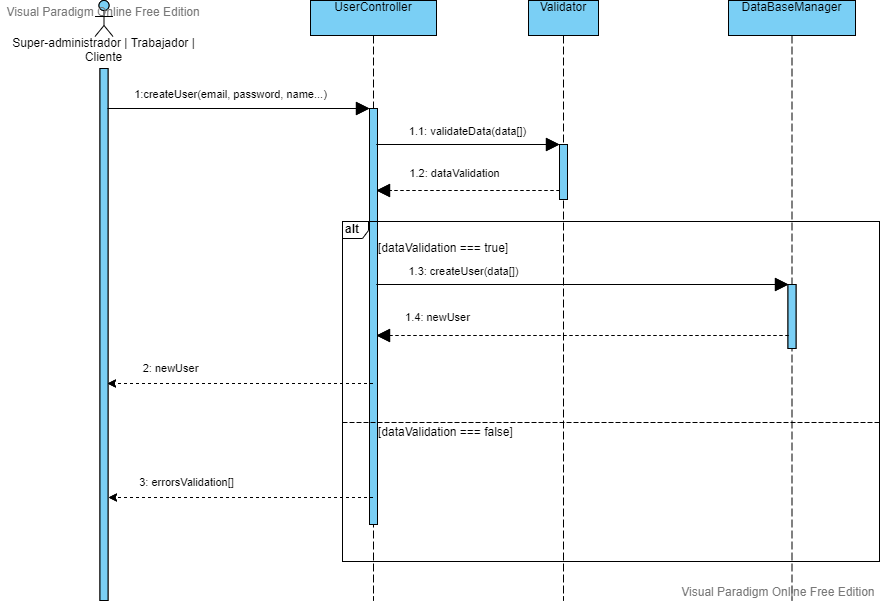
\includegraphics[scale=0.42]{images/Alta_Usuario.png}
  \caption{DS: Alta de cliente, trabajador o super-administrador.}
  \label{DS1}
\end{figure}

\begin{figure}[H]
  \centering
  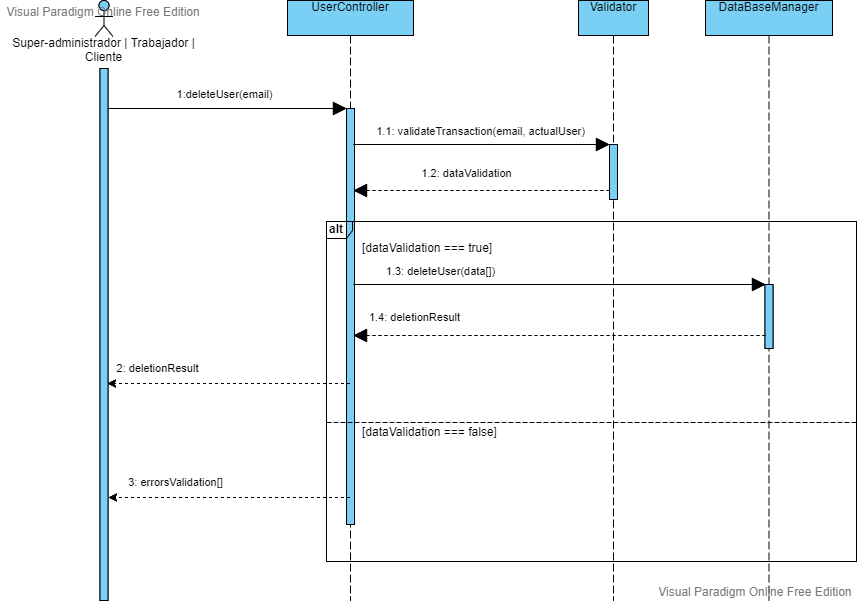
\includegraphics[scale=0.42]{images/Baja_Usuario.png}
  \caption{DS: Baja de cliente, trabajador o super-administrador.}
  \label{DS1}
\end{figure}

\begin{figure}[H]
  \centering
  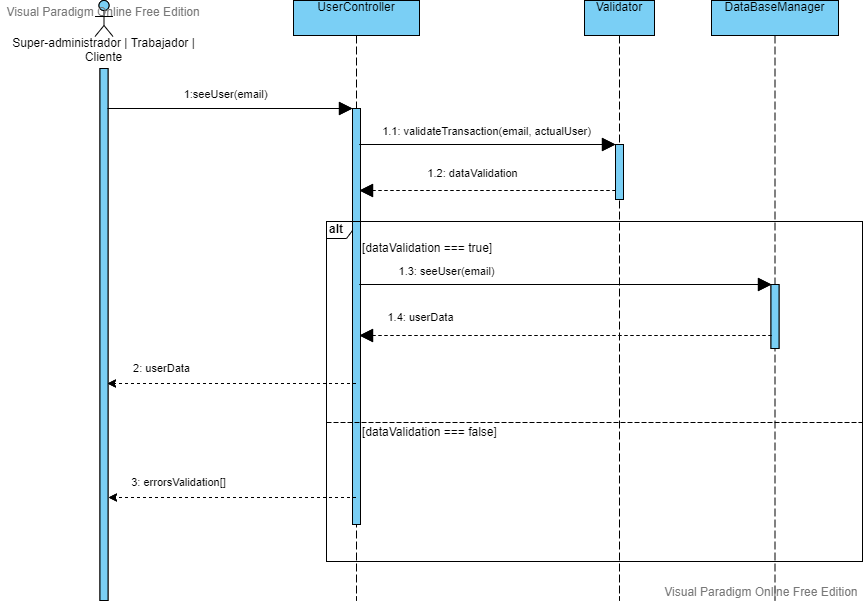
\includegraphics[scale=0.42]{images/Consultar_Datos_Usuario.png}
  \caption{DS: Consultar datos de cliente, trabajador o super-administrador.}
  \label{DS1}
\end{figure}

\begin{figure}[H]
  \centering
  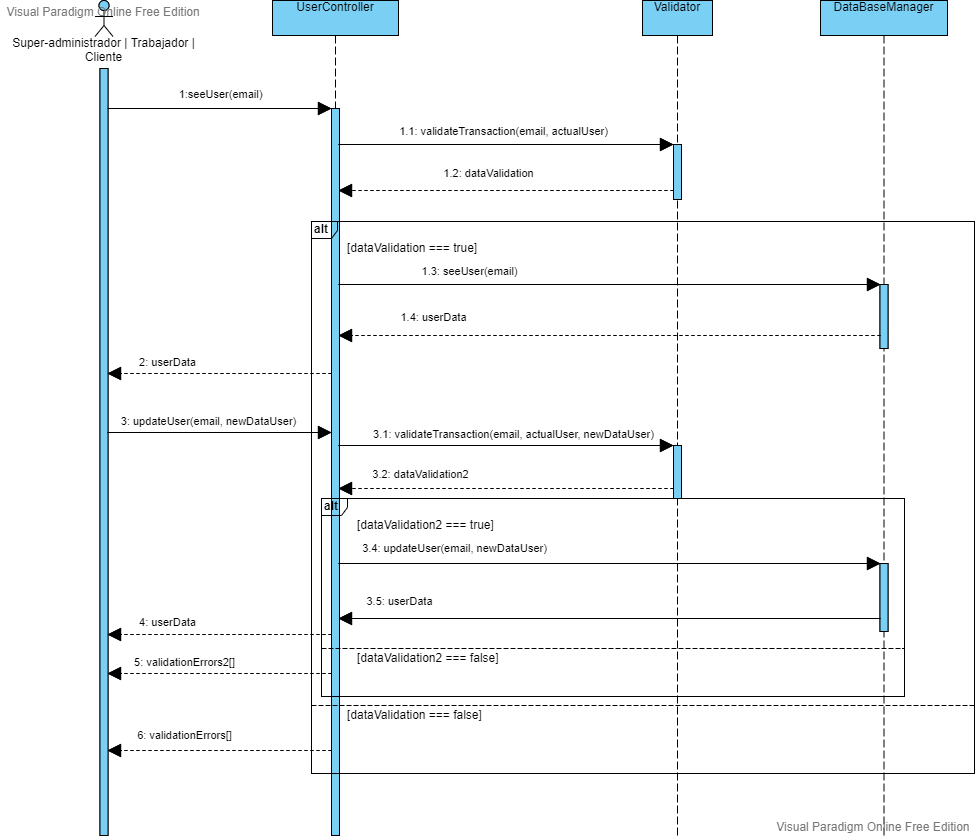
\includegraphics[scale=0.38]{images/Modificar_Datos_Usuario.png}
  \caption{DS: Modificar datos de cliente, trabajador o super-administrador.}
  \label{DS1}
\end{figure}

\begin{figure}[H]
  \centering
  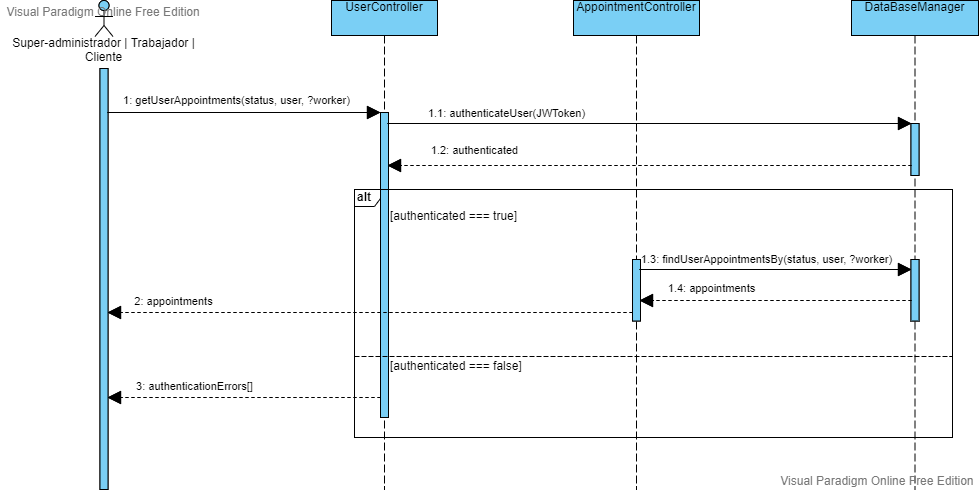
\includegraphics[scale=0.38]{images/Consultar_citas.png}
  \caption{DS: Consultar citas por cliente, trabajador o super-administrador.}
  \label{DS1}
\end{figure}

\begin{figure}[H]
  \centering
  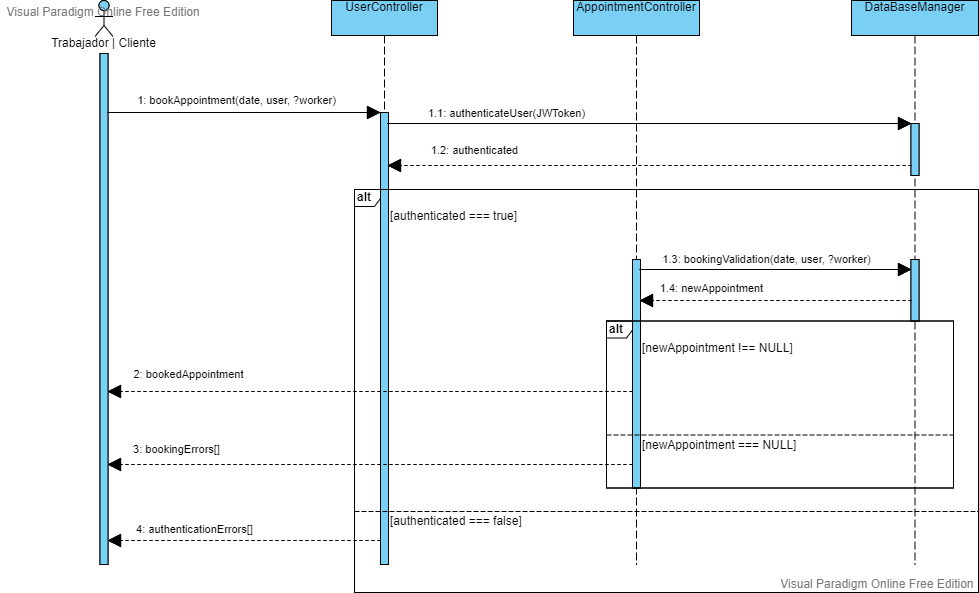
\includegraphics[scale=0.36]{images/Rerservar_cita.png}
  \caption{DS: Reserva de cita por cliente o trabajador.}
  \label{DS1}
\end{figure}

\begin{figure}[H]
  \centering
  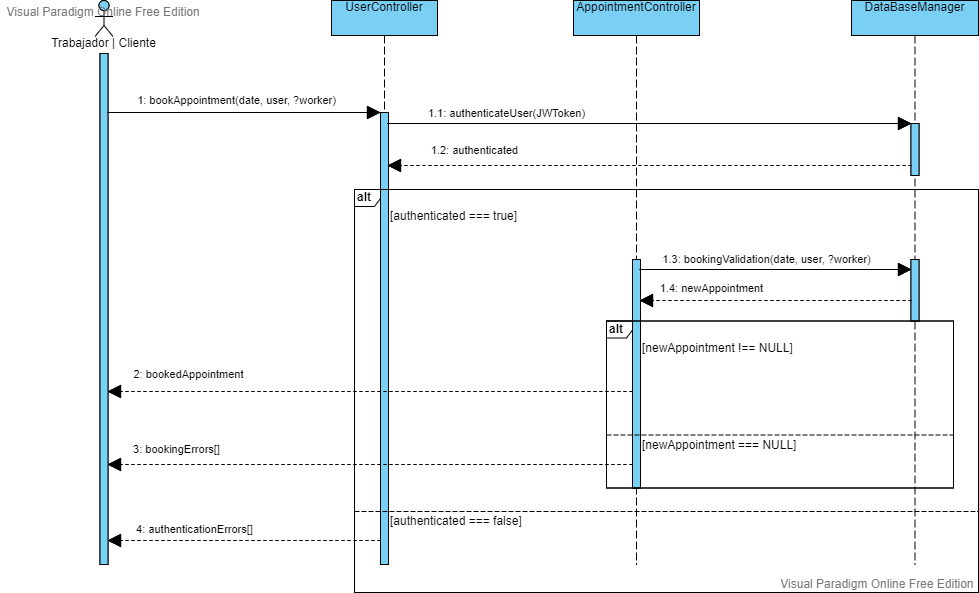
\includegraphics[scale=0.36]{images/Rerservar_cita.png}
  \caption{DS: Cancelación de cita por cliente o trabajador.}
  \label{DS1}
\end{figure}


\begin{figure}[H]
  \centering
  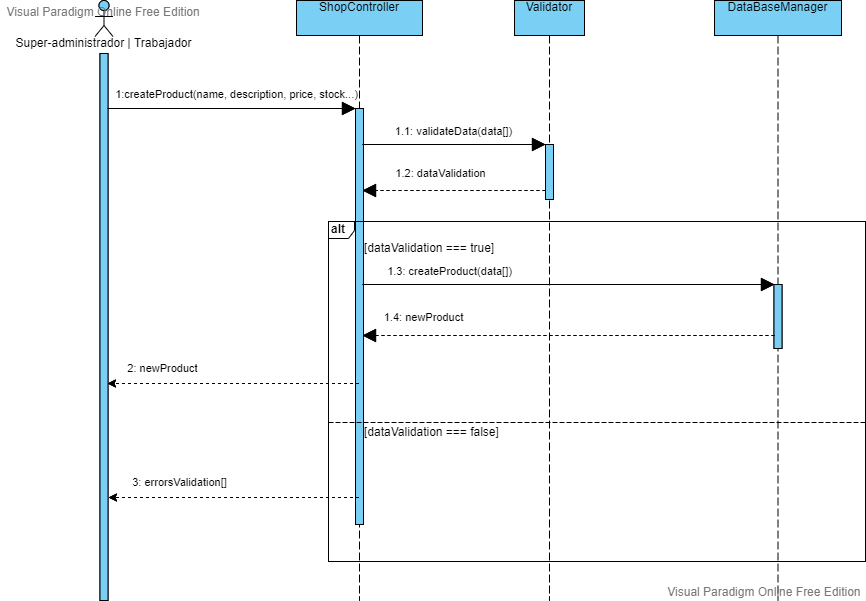
\includegraphics[scale=0.38]{images/Alta_Producto.png}
  \caption{DS: Alta de producto para venta online por trabajador o super-administrador.}
  \label{DS1}
\end{figure}

\begin{figure}[H]
  \centering
  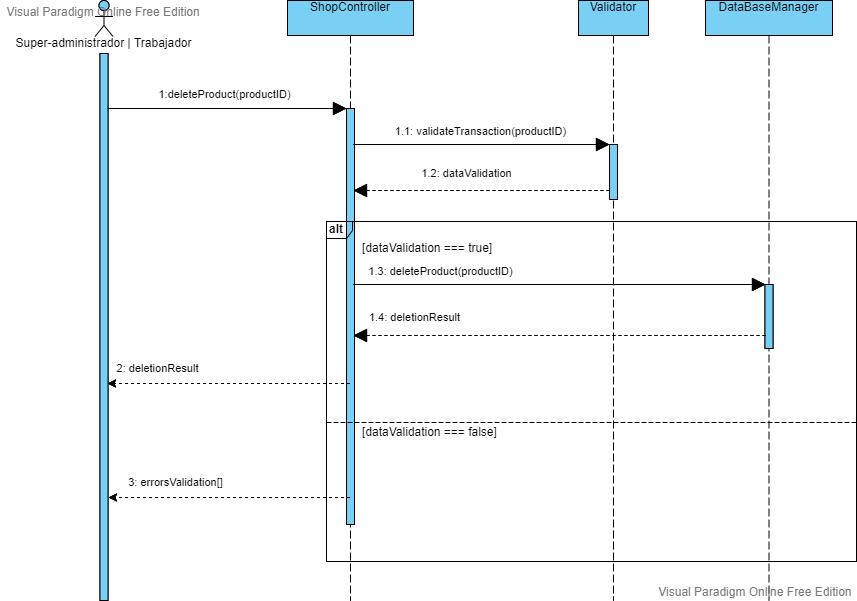
\includegraphics[scale=0.38]{images/Baja_Producto.png}
  \caption{DS: Baja de producto para venta online por trabajador o super-administrador.}
  \label{DS1}
\end{figure}

\begin{figure}[H]
  \centering
  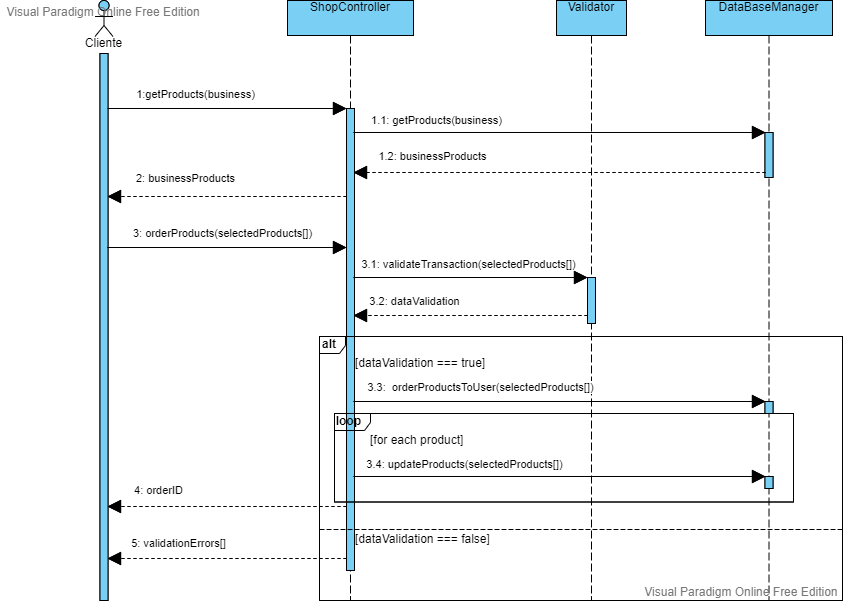
\includegraphics[scale=0.42]{images/Realizar_Pedido.png}
  \caption{DS: Realizar pedido de productos por cliente.}
  \label{DS1}
\end{figure}

\begin{figure}[H]
  \centering
  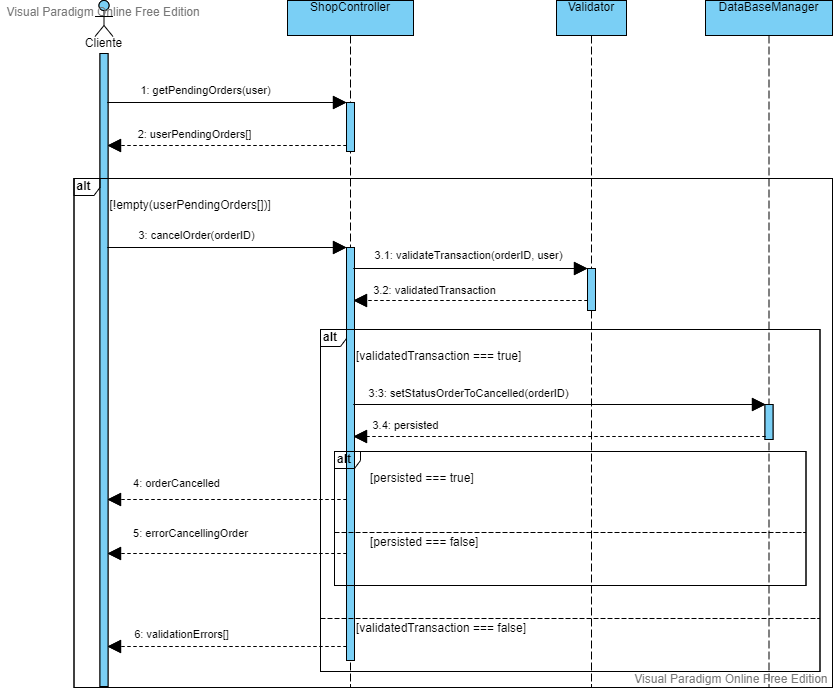
\includegraphics[scale=0.42]{images/Cancelar_Pedido.png}
  \caption{DS: Cancelar pedido por cliente.}
  \label{DS1}
\end{figure}

\begin{figure}[H]
  \centering
  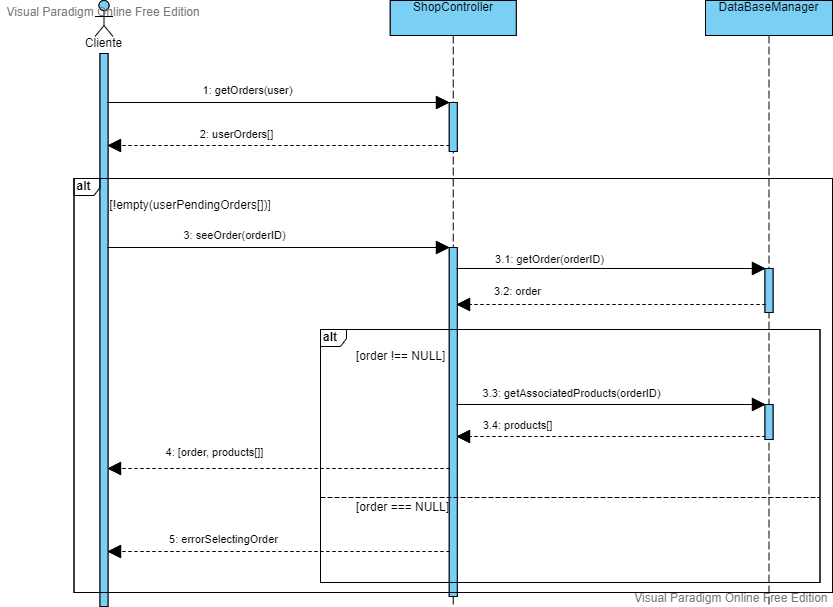
\includegraphics[scale=0.42]{images/Consultar_Pedido.png}
  \caption{DS: Consultar pedido de productos por cliente.}
  \label{DS1}
\end{figure}




    
    % Implementación
	\input{secciones/06_diseño}
	
    % Implementación
	\chapter{Implementación}

La implementación del software se ha dividido en hitos. Estos, han sido definidos en Github
y cada uno de ellos contiene un grupo de \textit{issues} que se corresponden con las distintas
mejoras que se han ido incorporando al software a lo largo de su desarrollo.\\

// TODO seccionar en toma de decisiones (tecnologias, bibliotecas, etc), 



	% Presupuesto

	% Conclusiones
	\chapter{Conclusiones y trabajos futuros}

\section{Temporización final}

\section{Objetivos alcanzados}

\section{Aprendizaje}

\section{Desarrollo futuro}

	% Trabajos futuros


	
	\newpage
% 	\bibliography{bibliografia}
    \printbibliography[nottype=misc]
    % \bibliographystyle{unsrt}


    \defbibheading{web}{\section*{Páginas de consulta}}
    \printbibliography[type=misc,heading=web]
	
\end{document}

